%% ============================================================
%%  Chapter 5 - Implementation and Experimental Results
%%  Implementation + results merged (ch6 dropped).
%%  Figures use the \IfFileExists fallback pattern from ch4 
%%  drop real files into figures/ to replace the placeholders.
%%  Citation keys reused: sharafaldin2018cicids.
%%  Full 79-feature table lives in Appendix A.
%% ============================================================

\chapter{Implementation and Experimental Results}
\label{chap:results}

\section{Introduction}
\label{sec:results_intro}

The previous chapter designed a system and explained why it was a good choice. This chapter completes that system design, and quantifies what it do es to unseen data. Since the justification is made with the benchmark, the system details will make it easier to assess those claims, we make two separate reports for what the system achieves: the first reports on a widely known public benchmark, the second will describe the results of our own laboratory traffic test.

And it's in the second part of that validation where this work comes out strongest. Anybody can train a classifier to work well on a known problem set or a benchmark. It's much more difficult and much more meaningful to see whether that classifier would recognise an attack, if and when the attacker presented one in a form it's never been trained on. It turns out that the result of that evaluation the main point of this paper isn't what we thought it would be when we set out.

The building details which were deferred from chapter\ref{chap:conception} tools, versions and command exact appear in the text only when they are relevant to the result; a full record of commands is provided in the annexes. The full feature reference is located in Appendix\ref{app:features} so that it does not disturb the flow of the text.

% ─────────────────────────────────────────────────────────────
\section{Laboratory Implementation}
\label{sec:results_lab}

The two-machine layout shown in Section~\ref{sec:conception_environment} has been set up on one host machine running KVM .
Pop!\_OS (a variant of Ubuntu) is the host operating system. We can install the machines as virtualizations on Linux and thus use KVM directly as opposed to having a large desktop virtualization layer underneath it, the realistic design of Chapter~\ref{chap:conception} only picked KVM because of this practicality.

Two VMs are running within a private virtual network. VM1 is hosting an Ubuntu Server and doing two things as discussed previously: acting as a system hosting the victims (an Apache web server, an SSH service, and an FTP service), as well as playing host to the probing mechanism designed to observe the victims. The second machine, VM2, running Kali Linux, is providing the attacking utilities used to shape up the traffic required to pose an attack. 
These include Nmap, Hydra and hping3 to provide scanning, brute forcing and flooding features respectively. 
All these traffic passes through the two machines, along a single isolated network segment (the \texttt{ids-lab} network, \texttt{192.168.100.0/24}), and the two machines possess an additional network interface providing access to the Internet and carrying experimental-unrelated traffic only. Having the actual attack path restricted to an isolated segment ensures that the traffic captured using \texttt{tcpdump} on the attacker is precisely the target network traffic to analyze:

\begin{figure}[H]
  \centering
  \IfFileExists{figures/lab_topology.png}{%
    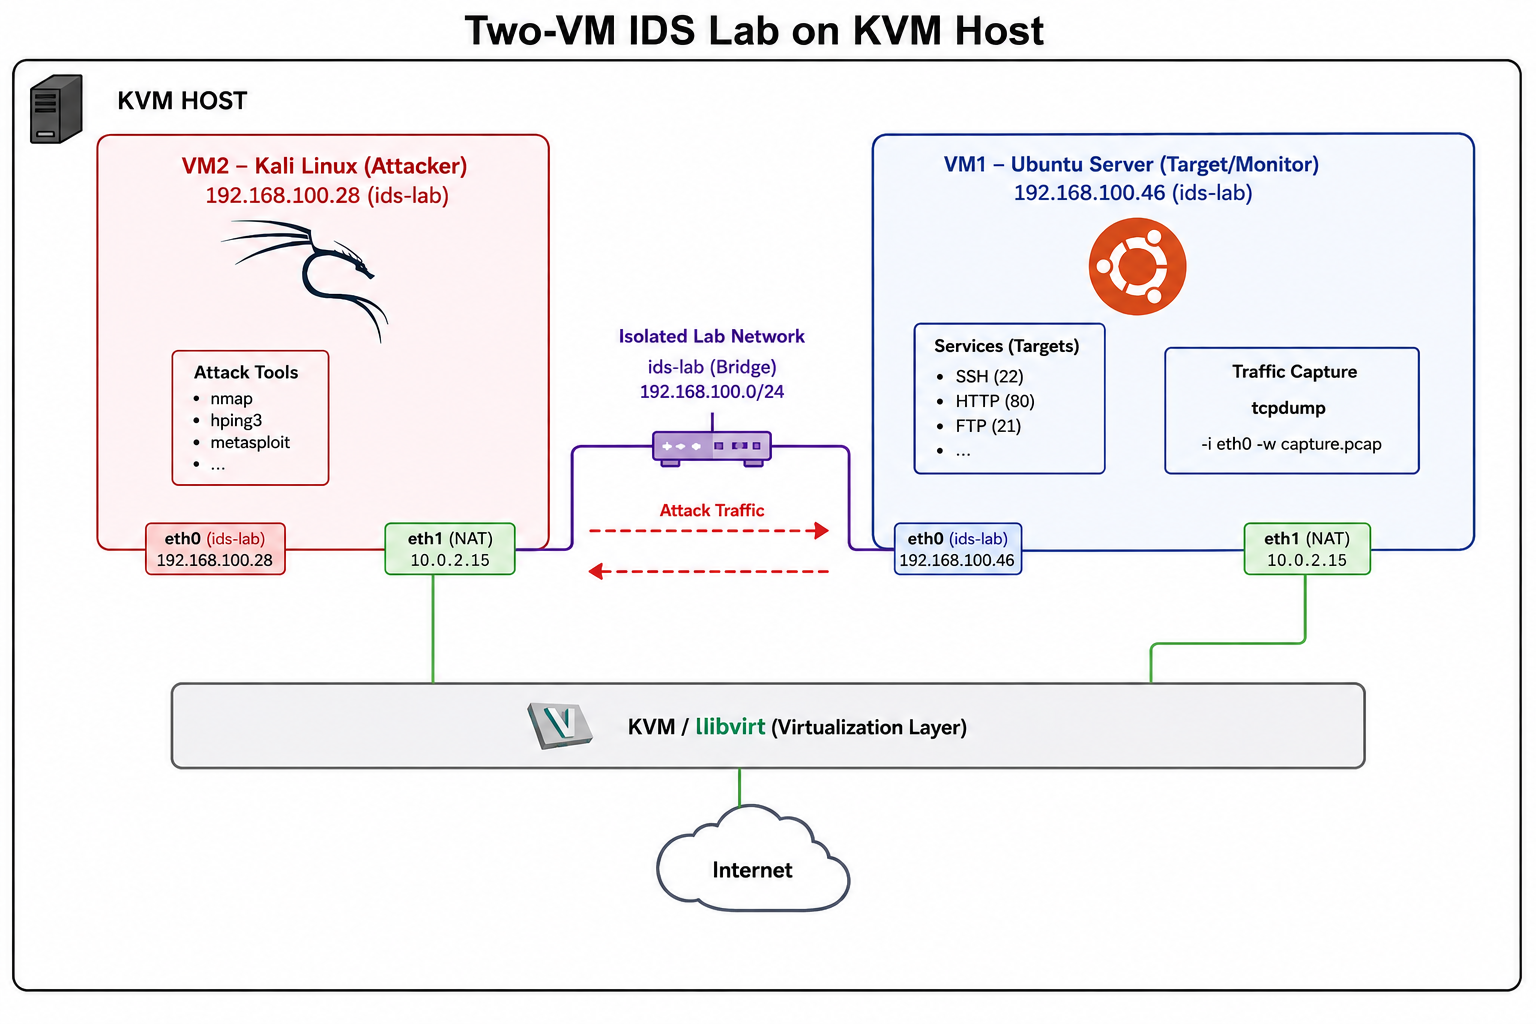
\includegraphics[width=0.9\textwidth]{figures/lab_topology.png}%
  }{%
    \fbox{\parbox{0.85\textwidth}{\centering\vspace{1.0cm}
    \texttt{[Figure: lab\_topology.png]}\\[4pt]
    \small Two-VM lab on the KVM host. VM2 (Kali, 192.168.100.28) launches
    attacks across the isolated \texttt{ids-lab} bridge toward VM1
    (Ubuntu Server, 192.168.100.46), which runs the target services and
    captures traffic with \texttt{tcpdump}. A second NAT interface on each VM
    provides internet access and carries no experimental traffic.
    \vspace{1.0cm}}}%
  }
  \caption{Realised two-machine laboratory on the KVM host.}
  \label{fig:lab_topology}
\end{figure}

We first ensured the system was set up to a known to a desired state before we moved to doing any scanning: that the two machines could reach one another across the segregated network, that the target services on VM1 returned requests, and that a traffic capture performed on VM1 with an attack against another machine (VM2) successfully captured the attack. With the environment established we were then ready for the rest of work!

% ─────────────────────────────────────────────────────────────
\section{Dataset Preparation}
\label{sec:results_dataset}

The detector is trained using \cite{sharafaldin2018cicids} the reasons of which are detailed in Section \ref{sec:conception_dataset}: it contains realistic traffic, it contains attack types that we want to experiment within the lab and the features file is also extracted using CICFlowMeter which the same as the tool which it is used live, thus, we maintain consistency of feature presentation. For the traffic captured within five days, we keep two days for training purposes; for the rest two days, we select six files for training purposes covering benign traffic, brute-force, Denial of service (DoS), web attack, Port Scanning and Distributed denial of service (DDoS); those other days, like “Infiltration” and “Botnet”, are excluded as demonstrated in Table \ref{tab:dataset_days}.

\subsection{Cleaning the raw feature files}
\label{sec:results_cleaning}

The released feature files are not of immediately use, and dealing with them threw up three specific issues that it would be good to record, since these also constitute work: 1. Column names: many rows containing column headers have leading spaces  for example “ Flow Duration” rather than “Flow Duration” ; the very first thing we have to do, therefore, is to trim white space from all column names, lest anything is refered to them by the wrong name. 2. Invalid numeric values: several of the features generated by CICFlowMeter are of the type rate bytes or packets per second and when the time duration of the flow being considered goes to 0, they write down an infinite value.

These infinite values make, however, it impossible to train any form of machine learning model, so we have opted to substitute them (positive and negative, individually) by a special missing value indicator and to remove any row with an infinity value. 3. Damaged label information for web-attack file: some attack names present in the original web-attack file have some illegal characters generated from some faulty encoding conversion, we clean-up such issue so that any row in the web-attack-traffic has a unique label. Furthermore (this one being a minor one compared to the others) they show a header row that is duplicated; we remove it at the same time in order to avoid an erroneous double counting of a features value.

Table~\ref{tab:cleaning_audit} records what each of these steps costs in flows, so that the size of the prepared dataset can be traced back to the released files.

\begin{table}[H]
  \centering
  \caption{Effect of each cleaning step on the number of flows.}
  \label{tab:cleaning_audit}
  \renewcommand{\arraystretch}{1.3}
  \begin{tabularx}{\textwidth}{Xrr}
    \toprule
    \textbf{Step} & \textbf{Flows removed} & \textbf{Flows remaining} \\
    \midrule
    Loaded from the eight released capture files & -       & 2,830,743 \\
    Rows holding an infinite or missing value    & 2,867   & 2,827,876 \\
    Exact duplicate flow records                 & 255,236 & 2,572,640 \\
    Flows labelled Infiltration or Bot           & 1,984   & 2,570,656 \\
    \midrule
    \textbf{Retained for modelling}              &         & \textbf{2,570,656} \\
    \bottomrule
  \end{tabularx}
\end{table}

Of the flows that remain, 16.5\% carry an attack label. Removing the duplicates is the step that matters most for the credibility of everything that follows: identical flow records falling on both sides of the train/test split would let the model be scored on rows it had already seen while training, which inflates every number reported later in this chapter.

\subsection{Label distribution and the imbalance problem}
\label{sec:results_imbalance}

The data, once combined, and washed clean, presents the class imbalance we suspected would result from our data collection process, from Chapter~\ref{chap:conception} that benign flows are largely in the majority, and combined across all attack types, we only have minority classes. Figure~\ref{fig:label_dist} demonstrates this. This is a typical class balance scenario where we will see that accuracy could trick the system, where a model that guesses every packet as benign still performs well for accuracy, yet detects nothing, which is why accuracy is presented in combination with recall, precision and F1, below.

\begin{figure}[H]
  \centering
  \IfFileExists{figures/label_distribution.png}{%
    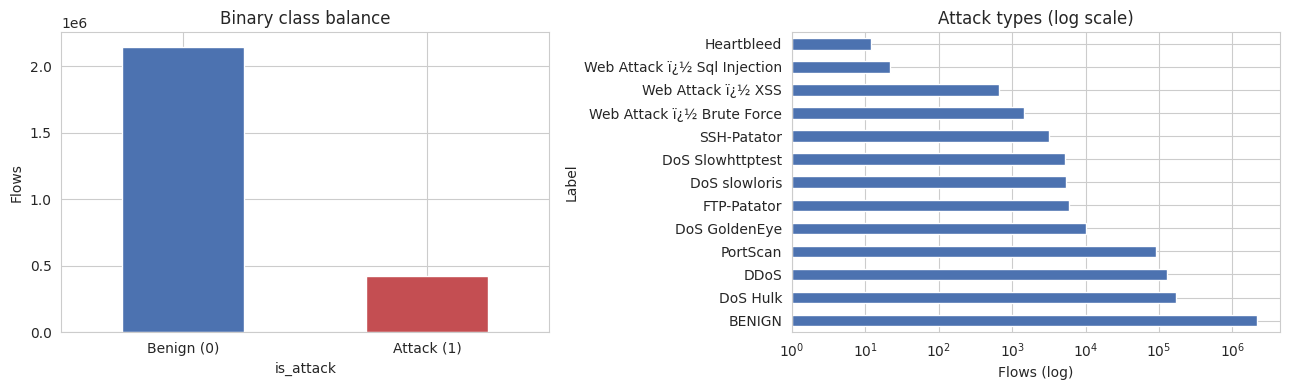
\includegraphics[width=\textwidth]{figures/label_distribution.png}%
  }{%
    \fbox{\parbox{1\textwidth}{\centering\vspace{4.0cm}
    \texttt{[Figure: label\_distribution.png]}\\[8pt]
    \small Class distribution across the six retained CICIDS-2017 files.
    Benign traffic forms the large majority; the attack classes
    (DoS, DDoS, PortScan, brute force, web attacks) form the minority,
    motivating imbalance-aware metrics and class weighting.
    \vspace{4.0cm}}}%
  }
  \caption{Distribution of benign and attack flows in the prepared dataset.}
  \label{fig:label_dist}
\end{figure}

From a different perspective, two different features offer the same view of the data. Figure~\ref{fig:eda_hist} shows the benign and attack distribution overlayed for flow duration and forward packet count. The attack distribution mostly overlies the benign distribution across most of the range, and the two separate only in the tails. This indicates we will need a learned model as this would require a very high sensitivity threshold to be manually defined and still not perform well. The signal is likely in the interactions of a set of features, not contained in a single feature, which is the goal for the candidates in Section~\ref{sec:results_models}.

\begin{figure}[H]
  \centering
  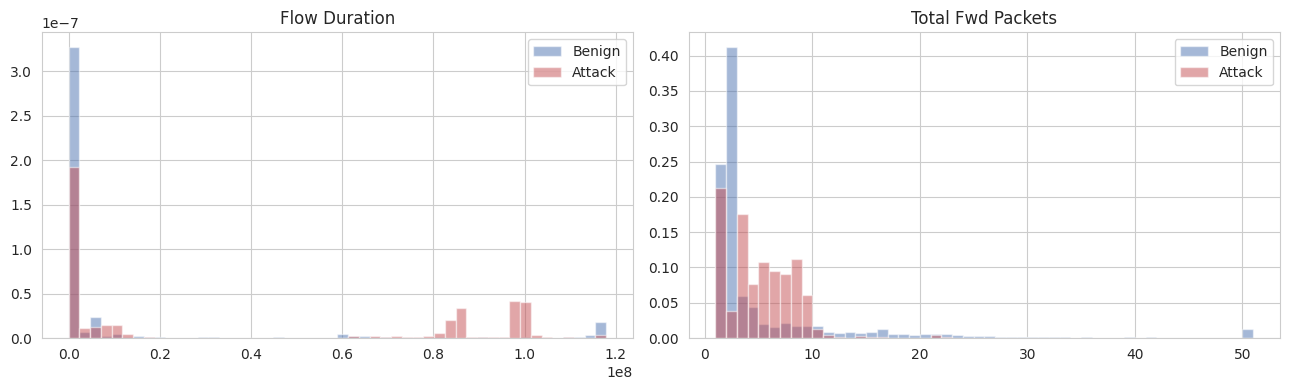
\includegraphics[width=\textwidth]{figures/eda_feature_histograms.png}
  \caption{Benign against attack distributions for two example features. Values are clipped at the 99th percentile and drawn as densities, so that the two very unequal class sizes stay comparable.}
  \label{fig:eda_hist}
\end{figure}

% ─────────────────────────────────────────────────────────────
\section{Feature Engineering and Selection}
\label{sec:results_features}

CICFlowMeter represents each flow using 79 features. Features can be grouped into several families of features: flow identifiers \& destination port, number of forward and backward packets and bytes, packet lengths statistics, inter-arrival time for flow, backward and forward direction, number of various tcp flags in flow, flow rates, connection-window and sub-flow characteristics. For instance, Flow Duration is feature counting the length of a connection, Total Fwd Packets number of packets moving toward forward direction, SYN Flag Count number of syn flags contained in the flow, or Flow Bytes/s represents amount of bytes carried in each direction within one second. Full list of CICFlowMeter's features is attached in Appendix~\ref{app:features} with brief definitions.

In addition we add 3 more engineered features those are features derived by explicitly forming a ratio that models a relationship that we either want the model to recognize easily or the model would likely fail to generalize properly, if we only rely on it inferring: ratio of forward to backward packets, ratio of forward to backward byte counts, and average forward packet size. They effectively codify a directional flow asymmetry to one value, something characteristic for a one sided flood as opposed to a balanced conversation.
 


Not all features have informativeness, for example, a few show almost equal values throughout the data and thus do not assist in discrimination. These features are subsequently removed through the use of a variance filter. This variance filter removed a total of eight columns, which contained equal values for each flow in the prepared dataset, namely the six bulk-transfer counters, backward PSH flag count and backward URG flag count.

The second layer of reduction is not the result of missing data but rather indicative of excessive redundancy. There appears to be (almost) duplicate values across the range of features, either because these features represent the same values under alternative names or because the features are simply a (non-unique) function of each other. Fig~\ref{fig:corr_heatmap} demonstrates the block structure of this correlation matrix.
When two variables are highly correlated (> 0.95) in the training split, one is discarded, which leads to the removal of a further 23 columns from the data set; see appendix~\ref{app:feat_dropped} for the names and duplicates of all removed features.
Two of the discarded features are particularly relevant to the next sections and are included here; the SYN flag count is discarded as the value is numerically the same as that of the forward PSH flag count for this data set, which means there is no SYN counter as an input to the deployed detector, and similarly for the ratio of the mean forward packet size (out of the three ratios that are engineered). Note that only two of the three ratios are used in the models. It can be seen from table~\ref{tab:feature_reduction} that the number of features is reduced stage by stage, ending at the 49 features that are used by the models, which the deep models then standardise before use.

\begin{table}[H]
  \centering
  \caption{Feature count at each stage of preparation.}
  \label{tab:feature_reduction}
  \renewcommand{\arraystretch}{1.3}
  \begin{tabularx}{\textwidth}{Xr}
    \toprule
    \textbf{Stage} & \textbf{Features} \\
    \midrule
    Numeric features in the released CSV files                      & 78 \\
    After removing the duplicated \texttt{Fwd Header Length} column & 77 \\
    After adding the three engineered ratios                        & 80 \\
    After the variance filter, (-8) constant columns                & 72 \\
    After the correlation filter, (-23) redundant columns           & \textbf{49} \\
    \bottomrule
  \end{tabularx}
\end{table}

\begin{figure}[H]
  \centering
  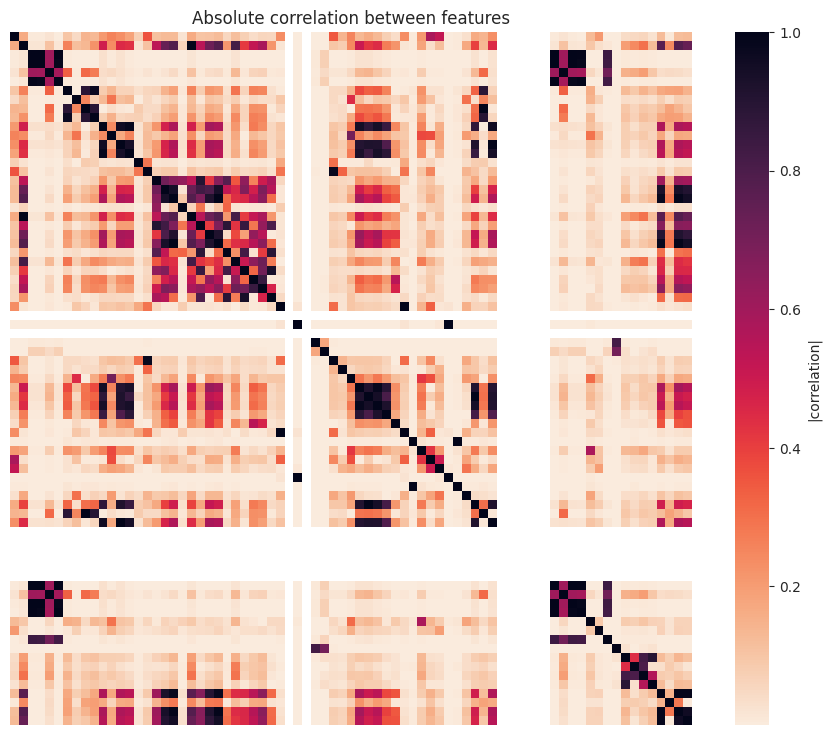
\includegraphics[width=0.82\textwidth]{figures/correlation_heatmap.png}
  \caption{Absolute correlation between the candidate features, on a sample of 300,000 flows. Axis labels are deliberately omitted; what matters is the block structure, each dark square being a group of features carrying nearly the same information.}
  \label{fig:corr_heatmap}
\end{figure} 


These 49 features are preserved along with their order alongside the model. It is important that the features given to the model are exactly those used during training.

The last detail to note is what is called order of operation. The details seem to be often glossed over but: all preparatory steps that learn anything from data; namely applying the variance filter, feature scaling as required for deep models, and resampling for balancing classes of training data; are determined on the training set only. Applying these steps prior to splitting the training/testing data would let information flow from the test set into the training set and hence cause over-estimation of results.

% ─────────────────────────────────────────────────────────────
\section{Model Development and Comparison}
\label{sec:results_models}


Chapter~\ref{chap:conception} had required to train a set of candidate models instead of a single one, in order for the data to decide in the classical or deep learning dilemma. It was eventually decided to train three models: a Random Forest (classical method), a Convolutional Neural Networks (CNN) and a Long Short-Term Memory network (LSTM). These last two are deep learning models, the LSTM being more suitable for sequential data, which should theoretically be optimal when attackers embed data into the order of the packets. These training runs were performed off the lab machines, on a Google Colab GPU, to make a clear separation of concern, as explained in Section~\ref{sec:conception_offline}.
A single split of the data was performed before any training, shared by all three models, to ensure a fair comparison. The split was selected as detailed in table~\ref{tab:protocol}. The three models were trained on the same stratified subsample of the training data so that the comparison would not take too long on a free GPU.
After the training, models were tested on a validation sample obtained from the same data, not the test set.
The test set was only used in section~\ref{sec:results_benchmark} to make one assessment. Using the test set to decide which model was best would have caused a bias, which would have the effect of adding performance to the models in a meaningless way. Values for each model are summarized in table~\ref{tab:hyperparams}.

\begin{table}[H]
  \centering
  \caption{Data partitions used for training, model selection and final evaluation.}
  \label{tab:protocol}
  \renewcommand{\arraystretch}{1.3}
  \begin{tabularx}{\textwidth}{Xrl}
    \toprule
    \textbf{Partition} & \textbf{Flows} & \textbf{Used for} \\
    \midrule
    Training set, 80\%              & 2,056,524 & everything fitted from data \\
    \quad bake-off subsample        & 370,174   & training the three candidates \\
    \quad validation split          & 205,653   & choosing the winner and the threshold \\
    Test set, 20\%, held back       & 514,132   & one final evaluation of the winner \\
    \bottomrule
  \end{tabularx}
\end{table}

\begin{table}[H]
  \centering
  \caption{Configuration of the three candidate models. Every run uses seed 42.}
  \label{tab:hyperparams}
  \renewcommand{\arraystretch}{1.3}
  \begin{tabularx}{\textwidth}{lX}
    \toprule
    \textbf{Model} & \textbf{Configuration} \\
    \midrule
    Random Forest (bake-off) & 100 trees, unlimited depth, square root of the feature count considered per split, balanced class weights, unscaled inputs \\
    Random Forest (deployed) & 200 trees, otherwise identical, retrained on the full training set \\
    CNN  & two one-dimensional convolutions, 1 to 32 and 32 to 64 channels with kernel size 3, ReLU and batch normalisation, adaptive max pooling, dense layer of 64 units, dropout 0.3 \\
    LSTM & one LSTM layer of 64 hidden units reading the feature vector as the sequence dimension, dense layer of 32 units, dropout 0.3 \\
    Both deep models & Adam at learning rate $10^{-3}$, batch size 1024, at most 15 epochs, early stopping with patience 3, class-weighted cross-entropy, standardised inputs \\
    \bottomrule
  \end{tabularx}
\end{table}

The comparison on the validation split is given in Table~\ref{tab:model_comparison}. It is the unexpected answer Chapter~\ref{chap:conception} teased at: Random Forest not only keeps up with the two deep models, but it outperformes both on all interesting measures; additionally it is also far less expensive both in training and execution.

\begin{table}[H]
  \centering
  \caption{Candidate model performance on the validation split of CICIDS-2017.}
  \label{tab:model_comparison}
  \renewcommand{\arraystretch}{1.3}
  \begin{tabularx}{\textwidth}{Xccccc}
    \toprule
    \textbf{Model} & \textbf{Precision} & \textbf{Recall} & \textbf{F1} & \textbf{ROC-AUC} & \textbf{PR-AUC} \\
    \midrule
    Random Forest & \textbf{0.9973} & \textbf{0.9961} & \textbf{0.9967} & \textbf{0.9998} & \textbf{0.9986} \\
    CNN           & 0.8713 & 0.9931 & 0.9282 & 0.9986 & 0.9930 \\
    LSTM          & 0.8645 & 0.9889 & 0.9225 & 0.9979 & 0.9903 \\
    \bottomrule
  \end{tabularx}
\end{table}


Figure~\ref{fig:model_bars} visualizes the above three rows in a diagram and the confusion matrices in Figure~\ref{fig:cm_validation} show what is lost between those summary metrics. Expressed as a precision of 0.87 the gap in false alarms looks modest, but in absolute terms it is large, and the main effect is the additional burden on an analyst's workflows. For 205,653 flows during validation, all three models detected virtually all the attack flows, with a recall never falling below 0.988.
The difference is in the benign flows, where the random forest generated 93 false alarms, but the CNN generated 4,975 and the LSTM model 5,253, more than fifty times as many.
In terms of detection, this is not significant, but in terms of workload and the tradeoffs in the cost to the analyst, it is. In this context, we can also revisit the situation raised in Section~\ref{sec:ids_commercial} with respect to noisy detectors.

\begin{figure}[H]
  \centering
  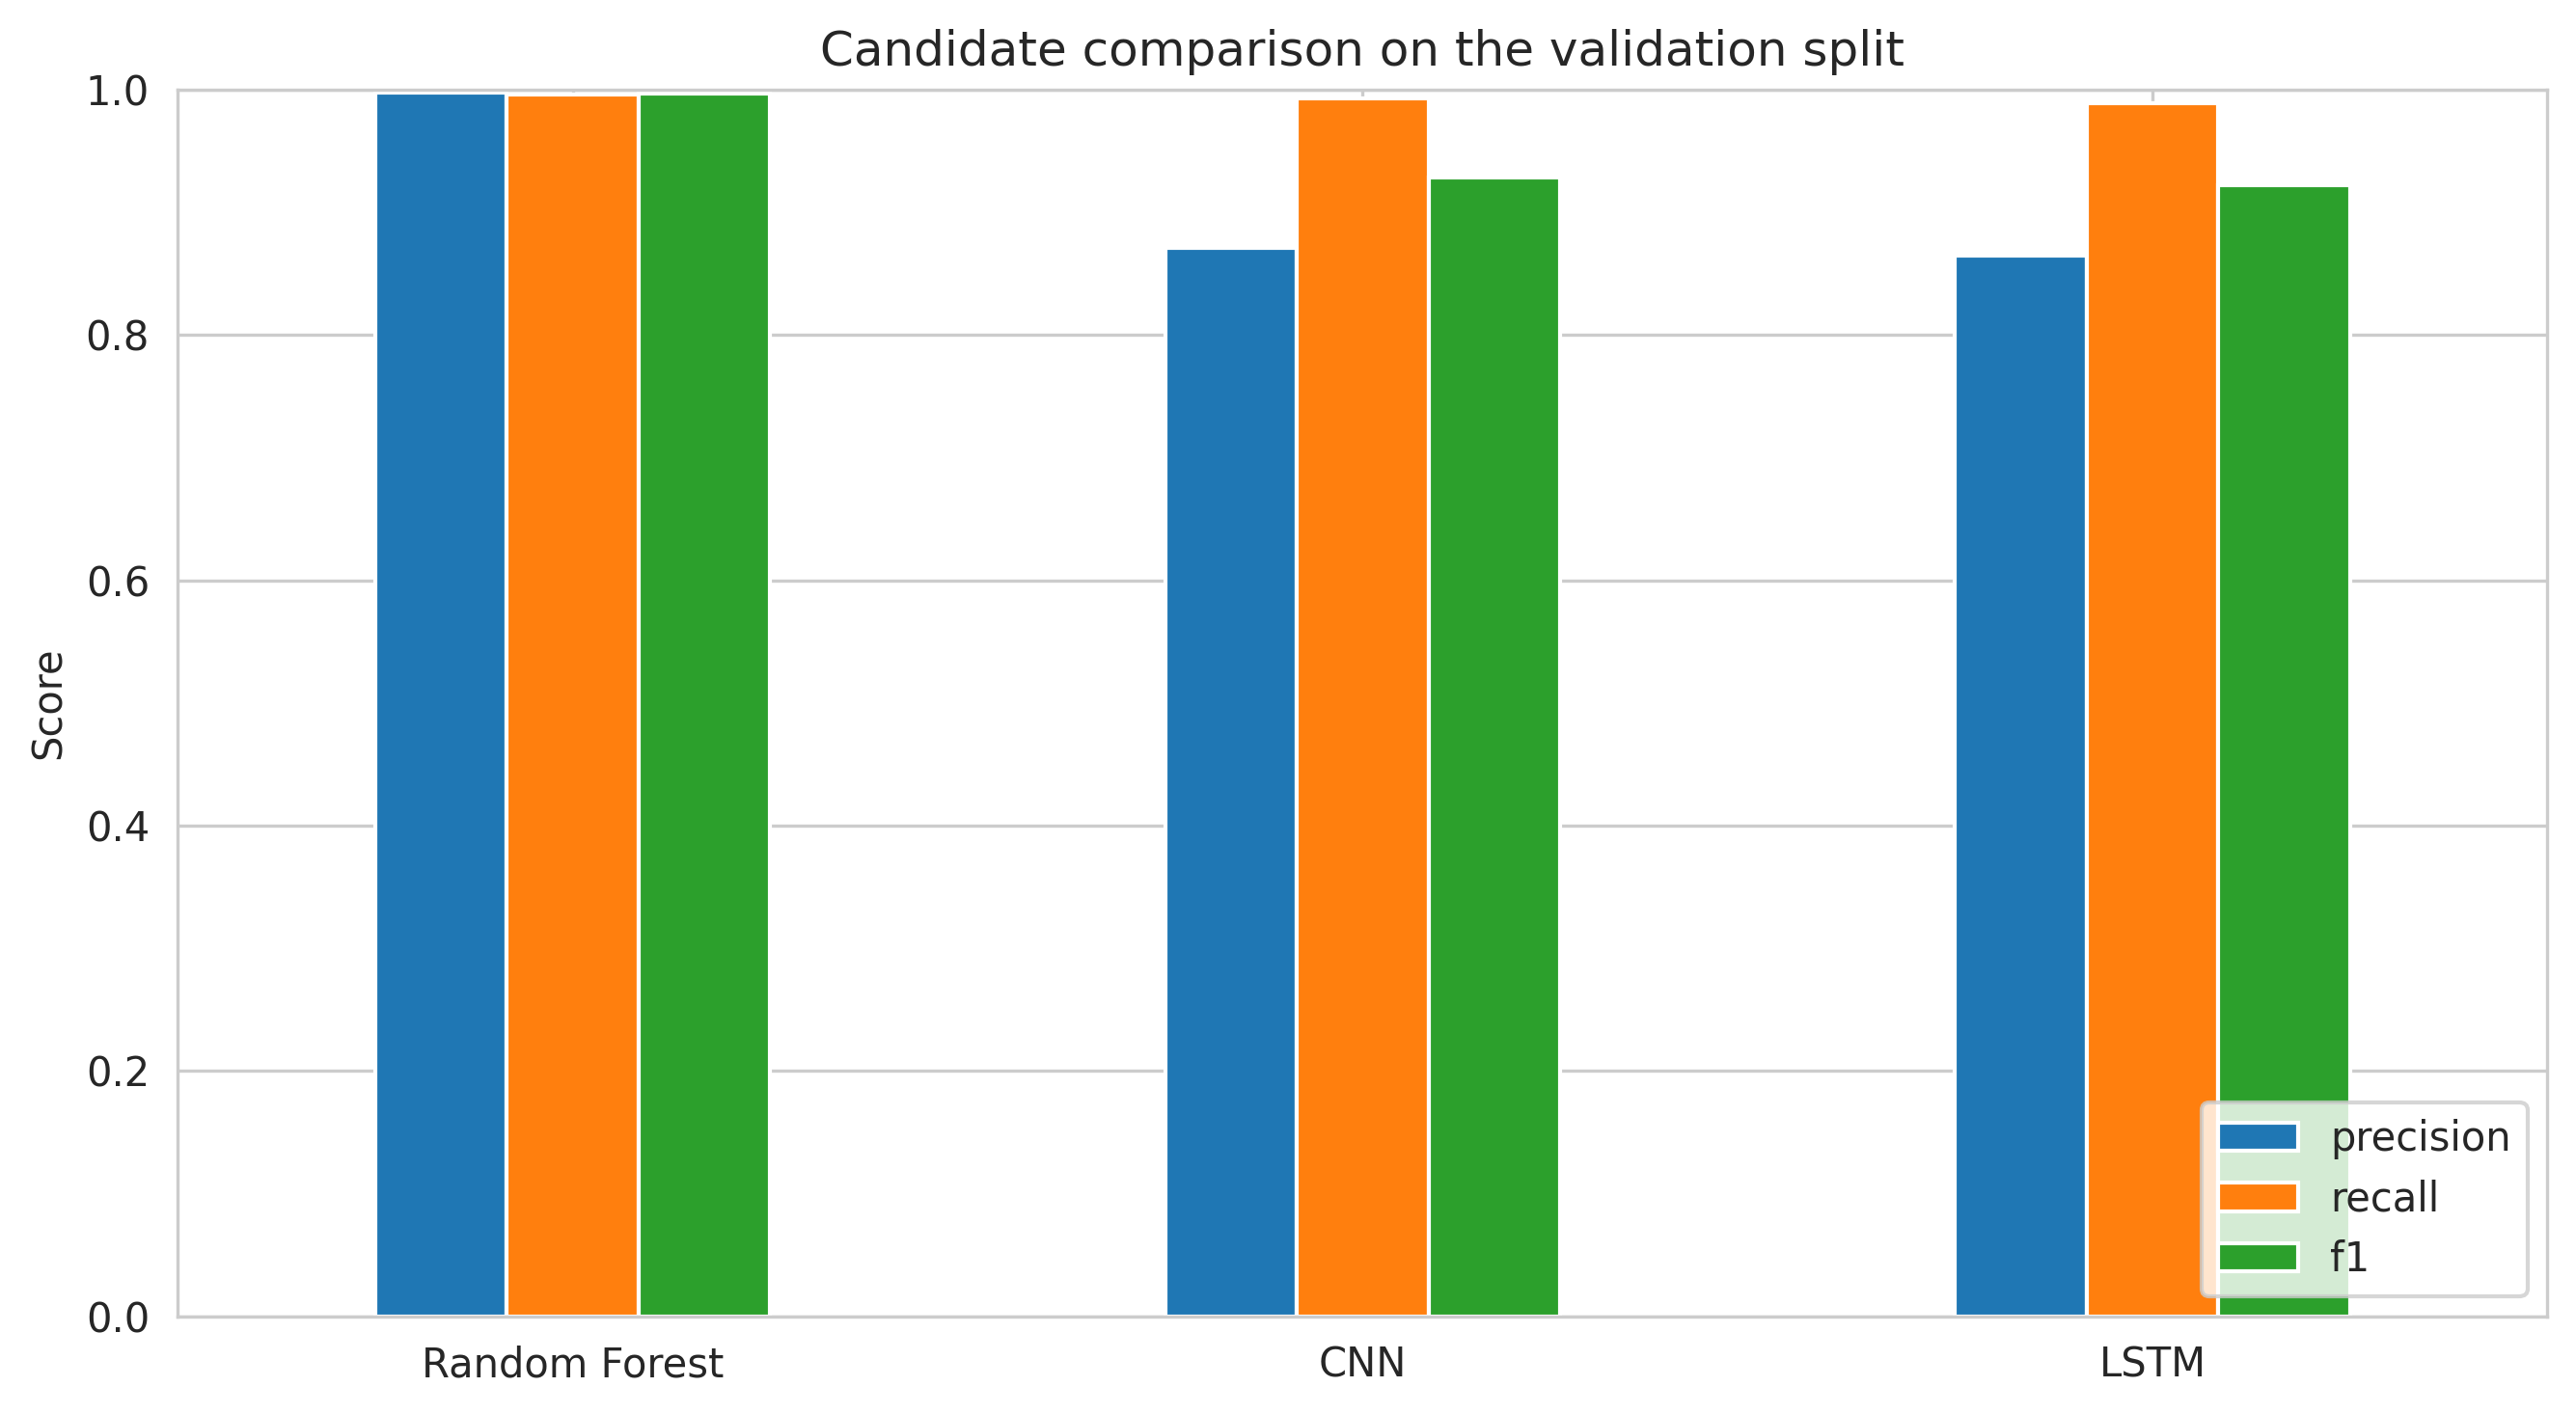
\includegraphics[width=0.85\textwidth]{figures/model_comparison_bars.png}
  \caption{Precision, recall and F1 of the three candidates on the validation split.}
  \label{fig:model_bars}
\end{figure}

\begin{figure}[H]
  \centering
  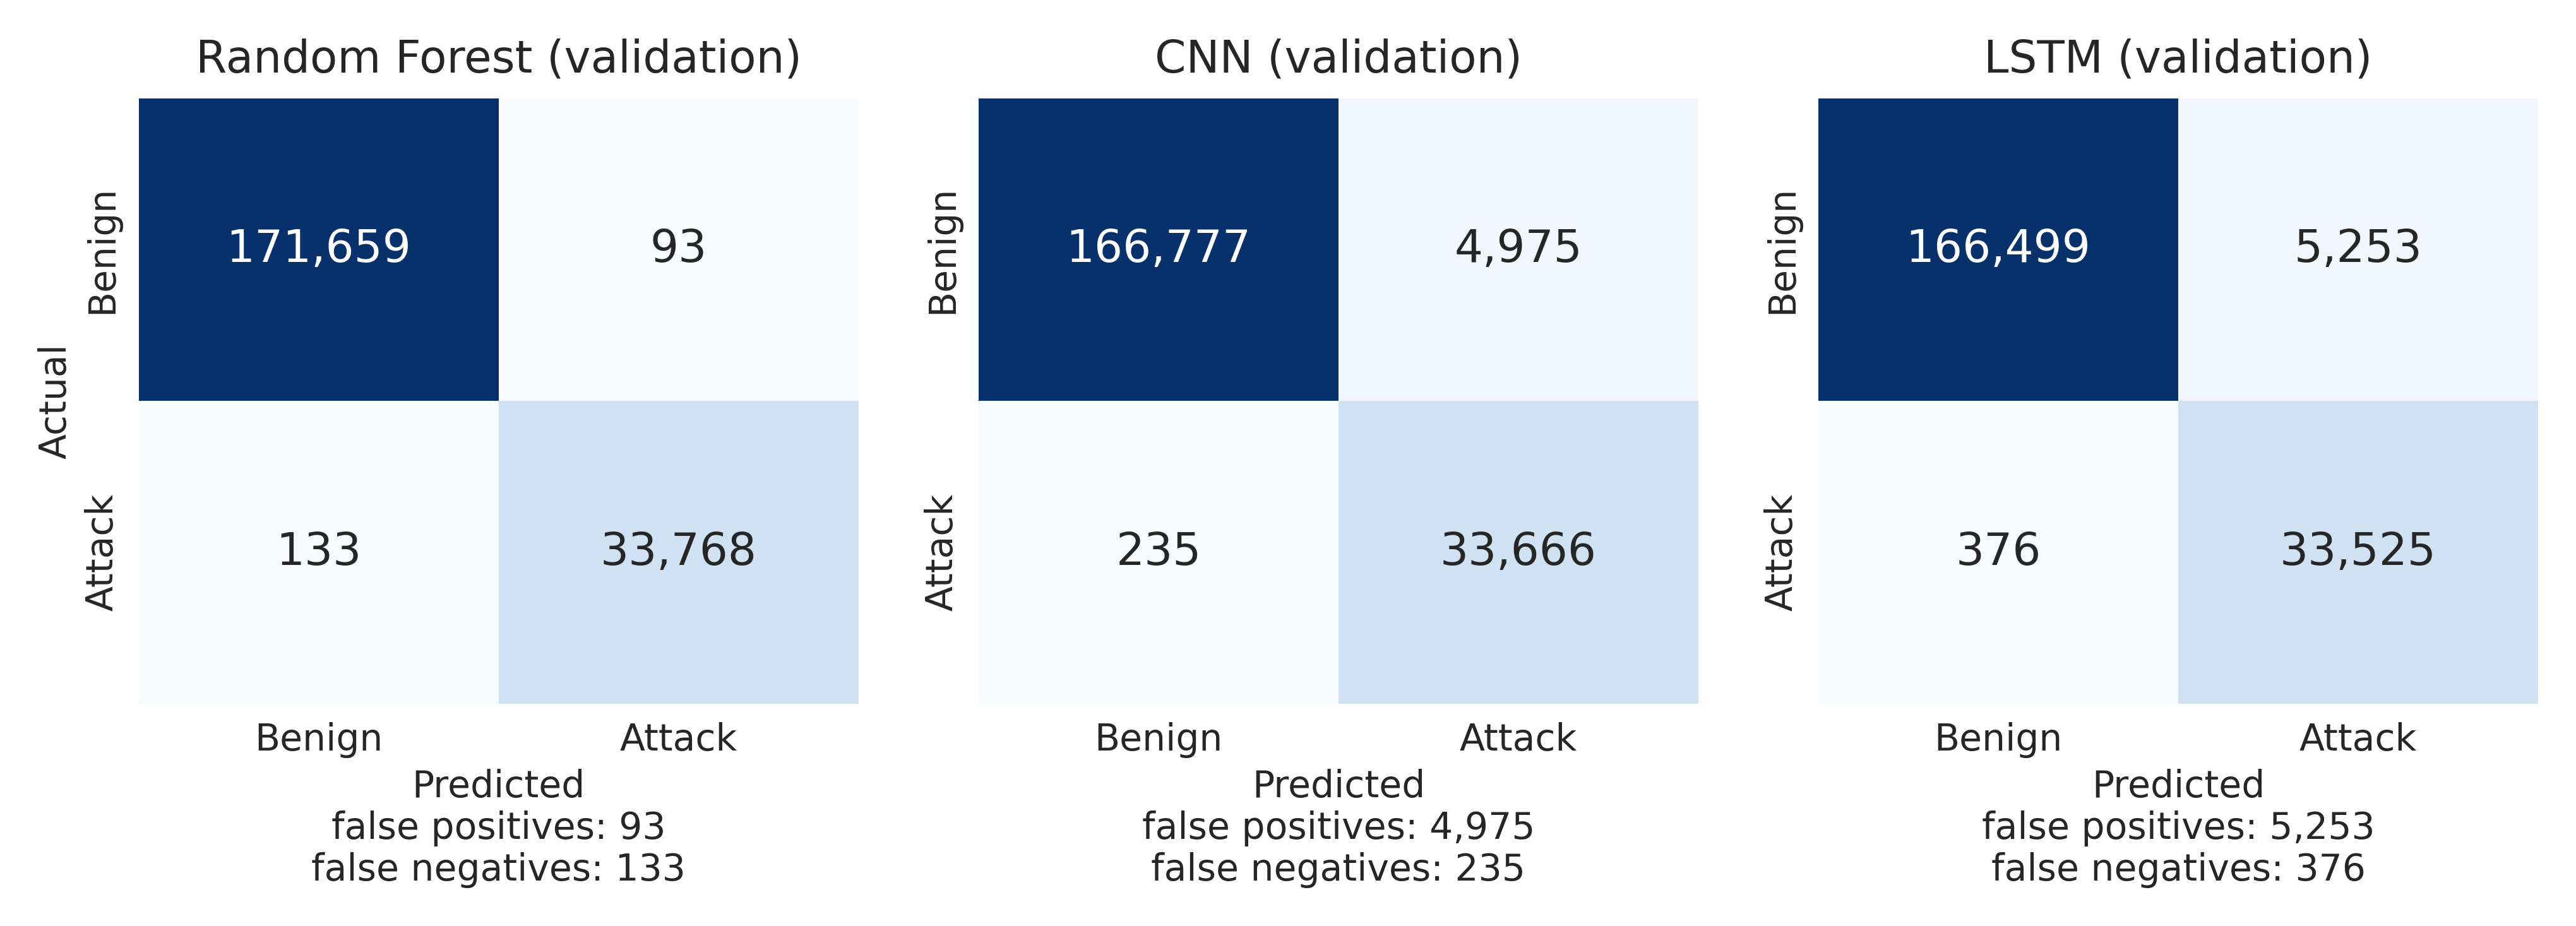
\includegraphics[width=\textwidth]{figures/cm_validation_three_models.png}
  \caption{Validation confusion matrices of the three candidates over the same 205,653 flows. The models are separated by their false-positive counts, not by their ability to catch attacks.}
  \label{fig:cm_validation}
\end{figure}

Perhaps this should not be as surprising as it seems, and this is what we would expect from Chapter~\ref{chap:ai}. For strong, already-reduced tabular features like these, it is very difficult to do better than the tree-ensemble models: they don’t require feature scaling, aren’t hurt by features with completely disparate scales, and don’t have the large, complex, precisely-tuned budgets required by deep learning models just to get to baseline. The deep models in our sample performed adequately overall; they hit our recall objective at the expense of additional false positives, and were far more computationally expensive to train ( and to operate: they consume more memory/CPU for inference). 
A detector we’re trying to run on a reasonably small machine could do better as a result of deploying a Random Forest: not only did it perform better but the overhead is low, and engineering costs low too. 
That doesn’t mean anything profound about deep learning models in general; only that that’s what we found for this job, on this data, which was the intention of Chapter~\ref{chap:conception}.

Using our chosen random forest, we tuned the decision threshold to values other than one half. Since the penalty for failing to detect an attack is different than the penalty for claiming there was an attack there was, a better model can be made by tuning threshold; our tuned threshold yielded the highest F1 on the validation set. The model we picked can class something like forty five thousand of these per second, which is the throughput necessary for real-time operation; it will crop up in the Discussion again.

% ─────────────────────────────────────────────────────────────
\section{Benchmark Evaluation}
\label{sec:results_benchmark}
 
On the held-out CICIDS-2017 data the winning Random Forest performs near flawlessly on the unseen data: F1 score $\approx 0.997$, ROC-AUC $\approx 0.9998$. Figure~\ref{fig:rf_confusion} shows the confusion matrix for this winning model, where almost every flow lands on the correct diagonal. In isolation, this would be more reason for skepticism than celebration, as a victory on a benchmark makes claims more about the benchmark itself than about real-world data.

\begin{figure}[H]
  \centering
  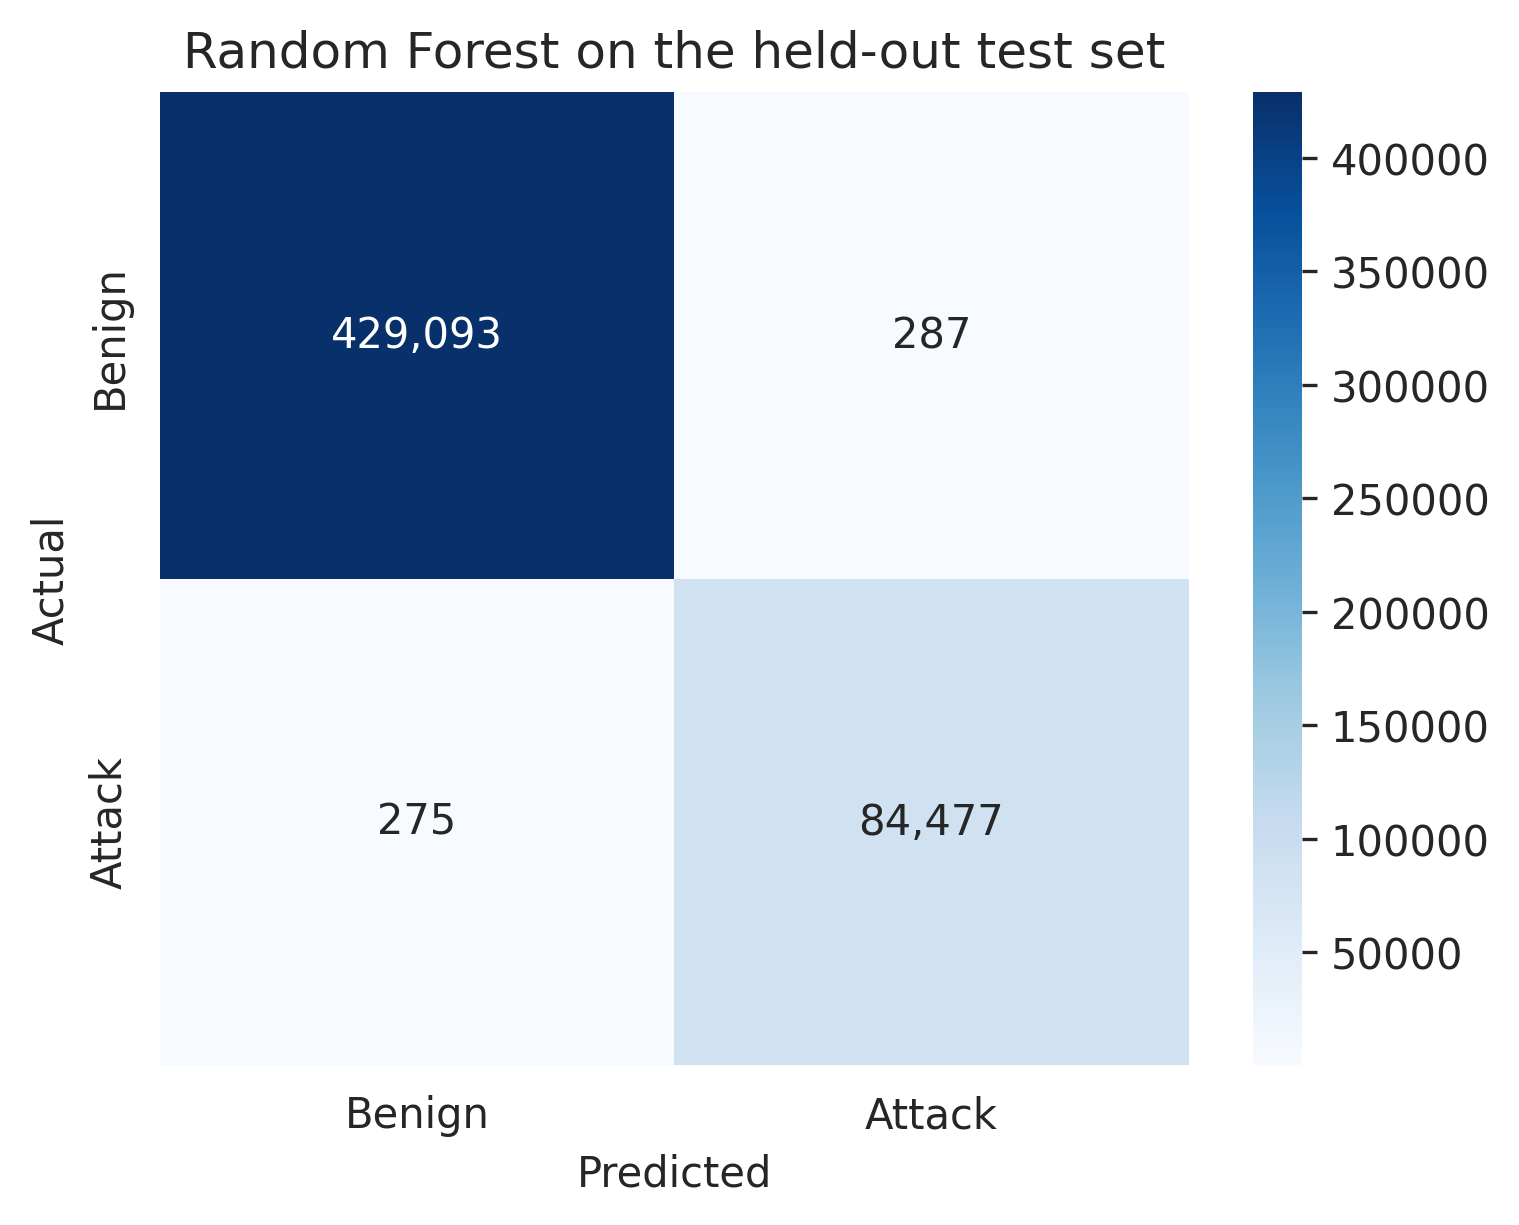
\includegraphics[width=0.62\textwidth]{figures/cm_rf_test.png}
  \caption{Confusion matrix of the deployed Random Forest on the held-out CICIDS-2017 test set.}
  \label{fig:rf_confusion}
\end{figure}

Of the total 514,132 test flows in total, out of which 287 benign flows are detected as attacks and 275 attacks are not detected when compared to 429,380 benign flows and 84,752 attacks. These four inferences are forming precision of 0.9966 and recall of 0.9968 in absolute values.


Since our dataset is imbalanced the precision-recall curve provides better insight than the ROC curve in our case: in a dataset dominated by normal traffic an ROC curve can show satisfactory results merely by the sheer number of correctly predicted negative values. The view on the precision-recall curve represents how accurately our attacks are being caught. Figure~\ref{fig:rf_pr} displays the PR curve of our finalized model over the test set, which identifies two points of operation-the default decision threshold of one half and the threshold we picked on the validation dataset (described in section~\ref{sec:results_models}). The PR curve also illustrates the tuning of decision threshold, yielding a slight decrease in one aspect when we chose to increase the other.
 
\begin{figure}[H]
  \centering
  \IfFileExists{figures/rf_pr_curve.png}{%
    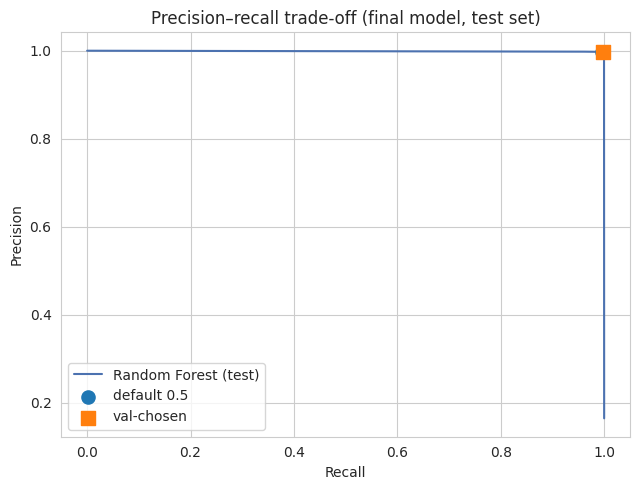
\includegraphics[width=0.7\textwidth]{figures/rf_pr_curve.png}%
  }{%
    \fbox{\parbox{0.85\textwidth}{\centering\vspace{1.0cm}
    \texttt{[Figure: rf\_pr\_curve.png]}\\[4pt]
    \small Precision--recall trade-off of the final Random Forest on the test
    set, with the default (0.5) and validation-chosen operating points marked.
    Exported from the training notebook.
    \vspace{1.0cm}}}%
  }
  \caption{Precision-recall trade off of the selected model, with both operating points.}
  \label{fig:rf_pr}
\end{figure}

Table~\ref{tab:operating_points} quantifies the two points. Changing the threshold from the default of 0.5 to the validation-split-selected threshold of 0.340 increases recall from 0.9968 to 0.9987; this recovers about 160 more attacks out of the 84,752, at a cost of three ten-thousandths of precision. This may be an acceptable tradeoff for a detection system. Both rows are shown because the threshold is an operating choice of the system operators rather than a property of the model itself.


\begin{table}[H]
  \centering
  \caption{Test-set performance of the deployed model at the two operating points marked in Figure~\ref{fig:rf_pr}.}
  \label{tab:operating_points}
  \renewcommand{\arraystretch}{1.3}
  \begin{tabularx}{\textwidth}{Xccc}
    \toprule
    \textbf{Decision threshold} & \textbf{Precision} & \textbf{Recall} & \textbf{F1} \\
    \midrule
    Default, 0.500                        & 0.9966 & 0.9968 & 0.9967 \\
    Chosen on the validation split, 0.340 & 0.9963 & \textbf{0.9987} & \textbf{0.9975} \\
    \bottomrule
  \end{tabularx}
\end{table}
 

The more subtle approach is to treat it as multi-class and not as a benign vs attack issue. In this context the model detects all high volume network attacks (DoS, DDoS, Port Scan, Brute Force) with near perfect accuracy but is clearly much less effective with web based attacks, where the cross-site scripting score is lower. This is of course what we might expect, the web attacks leave little trace in the flow statistics and closely resemble ordinary traffic, unlike the high volume attacks which are very different. Its a pretty straightforward benchmark for the obvious attacks but quite difficult for the less obvious which is surely the way the results should play out (and which will form the main point of the next section).


Figure~\ref{fig:cm_multiclass} and Table~\ref{tab:per_class} show the results in more detail. The results are promising, with 9 out of the 11 classes predicted almost perfectly, but the two web-attack classes are clearly hard to distinguish. The confusion matrix shows where the problem lies: 86 of the 130 cross-site scripting flows are predicted as web brute-force, while 60 brute-force flows are wrongly predicted as scripting.
This leads to a drop in the XSS F1 score to 0.36.
But these two classes look identical at the level of flow statistics: both have a short HTTP request to the same server and port, and nothing on the flow feature vector indicates whether the payload is a script or a password guess. The matrix also shows the only appreciable confusion outside the web classes, between benign flows and portscan, with 222 benign flows predicted as portscan and 159 portscan flows predicted as benign. Again, this is no surprise, as the attack and benign flows both use a very short connection and transfer very little data.

\begin{figure}[H]
  \centering
  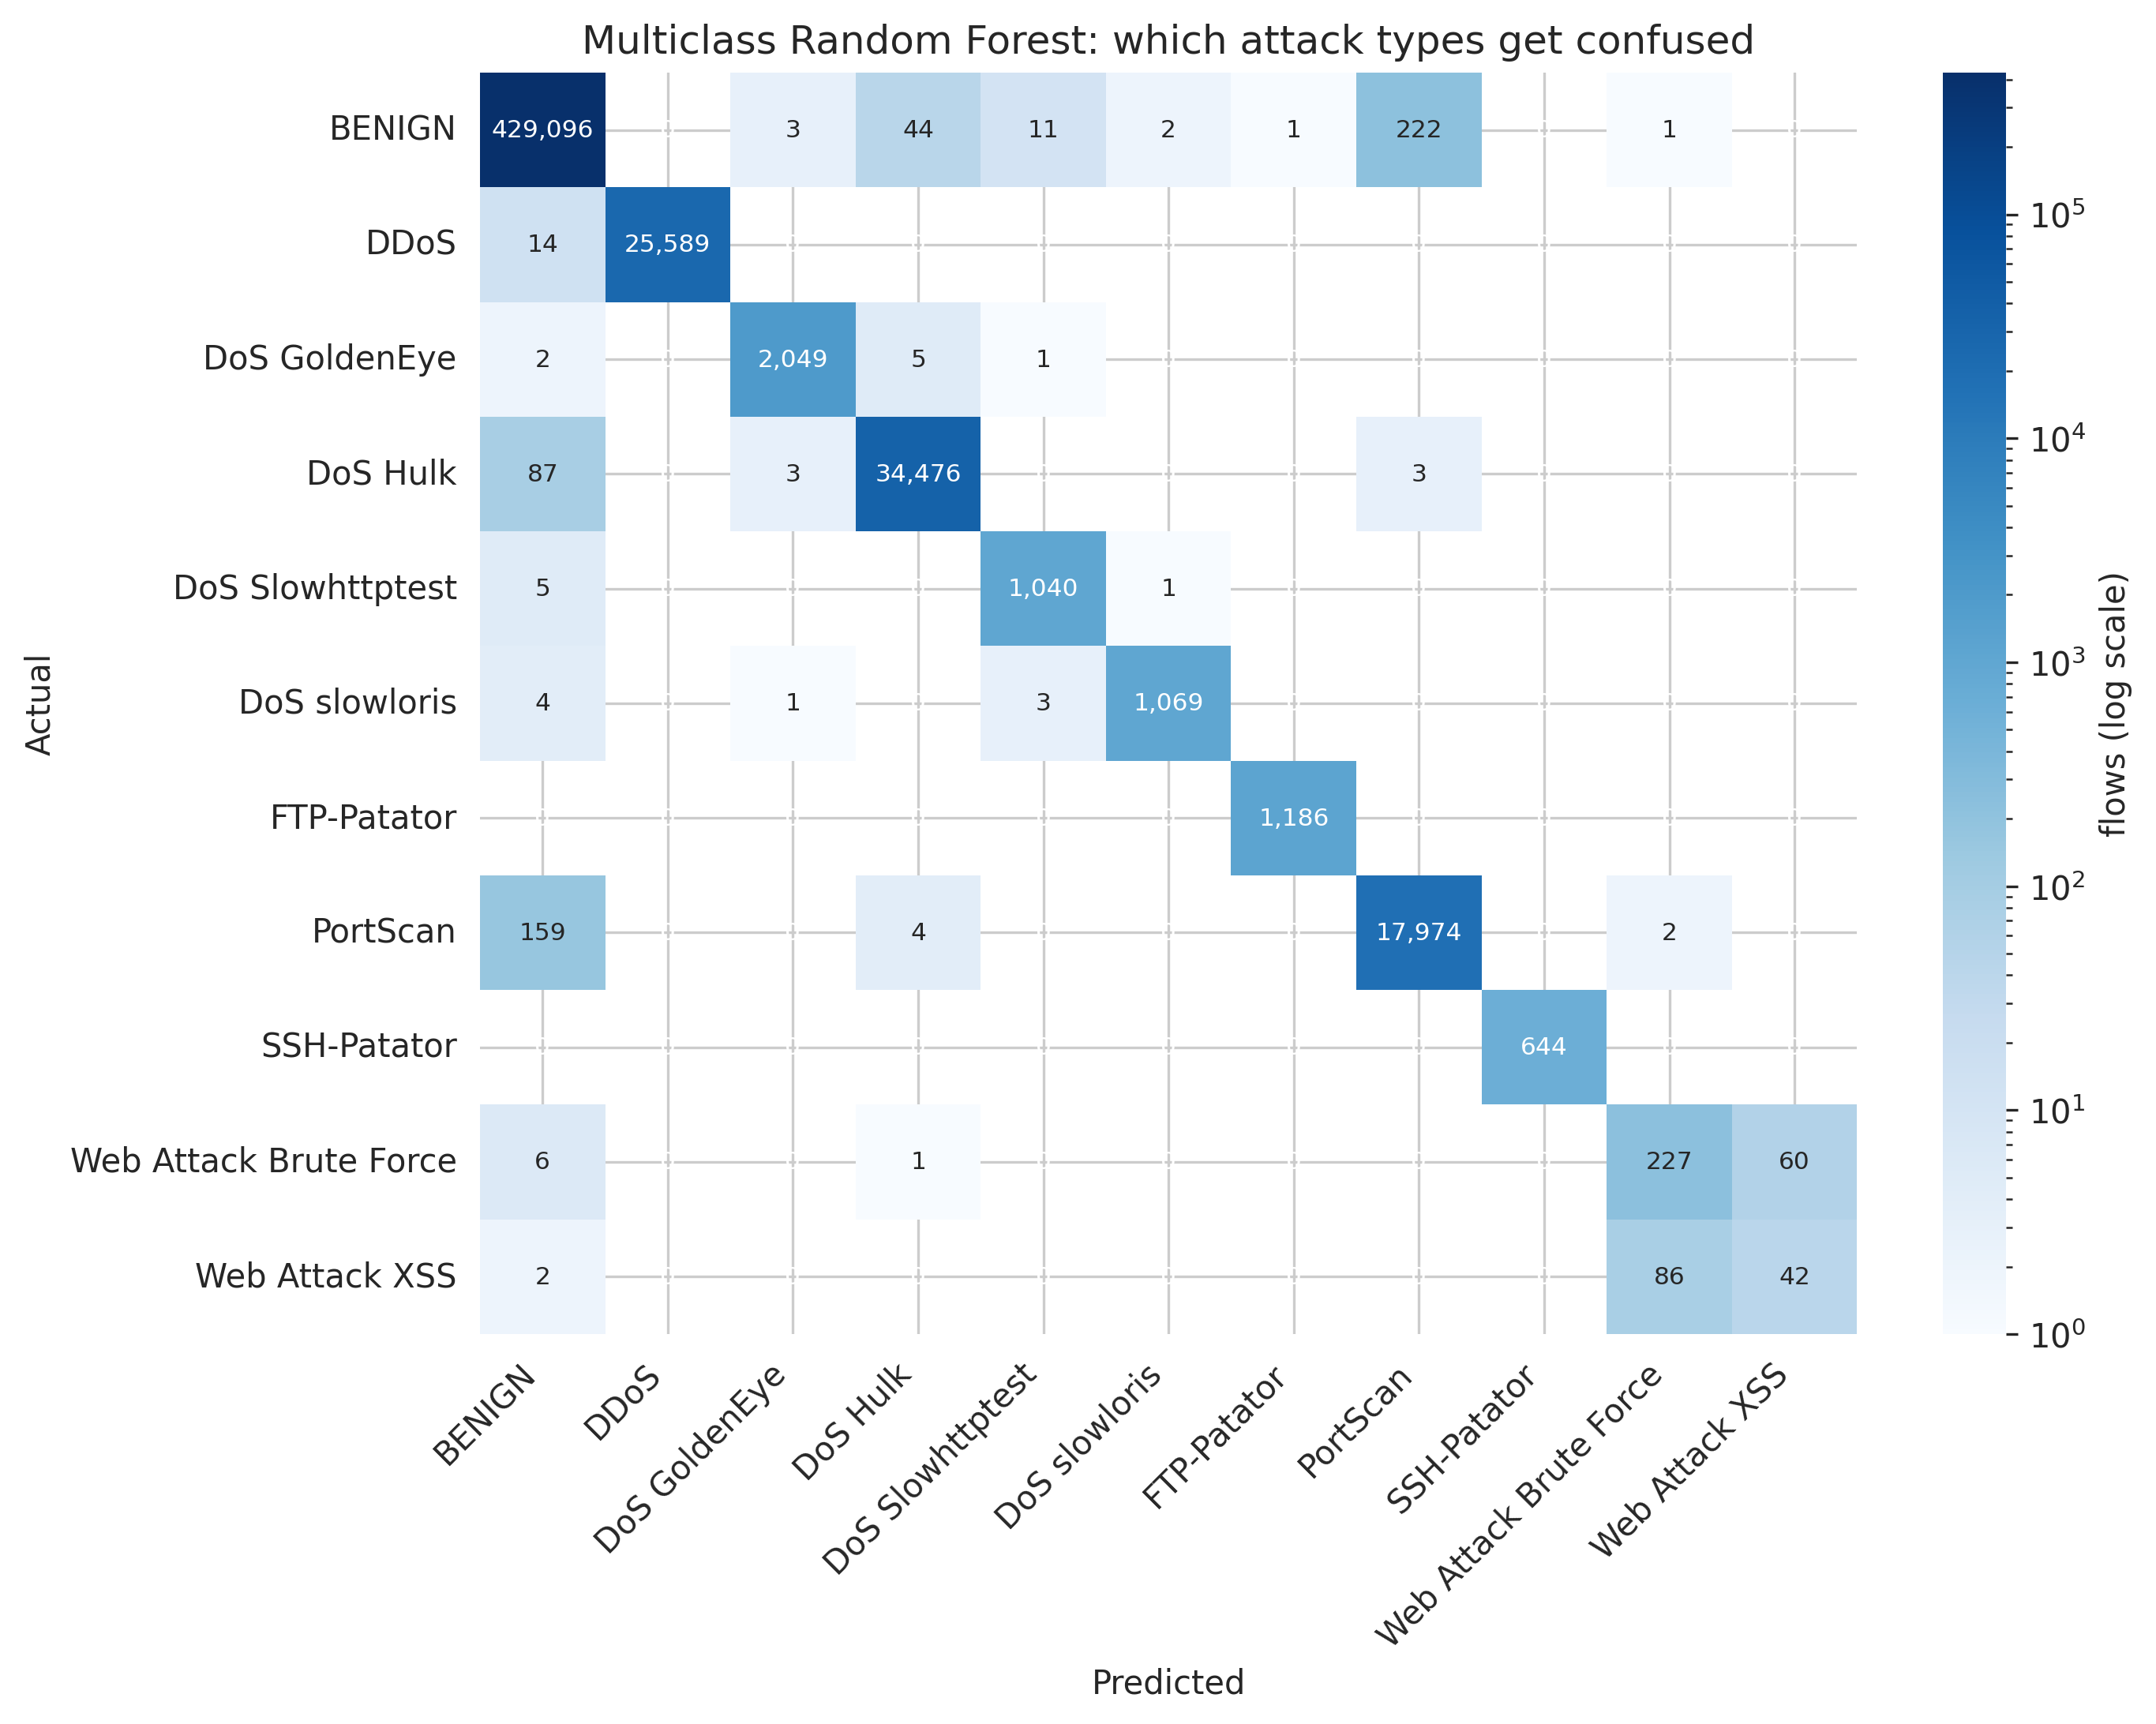
\includegraphics[width=0.86\textwidth]{figures/cm_multiclass.png}
  \caption{Confusion matrix of the multiclass Random Forest over the eleven retained attack types. The colour scale is logarithmic so that the small classes stay visible beside the benign class.}
  \label{fig:cm_multiclass}
\end{figure}

\begin{table}[H]
  \centering
  \caption{Per-class performance of the multiclass Random Forest on its held-out set.}
  \label{tab:per_class}
  \renewcommand{\arraystretch}{1.05}
  \begin{tabularx}{\textwidth}{Xcccr}
    \toprule
    \textbf{Class} & \textbf{Precision} & \textbf{Recall} & \textbf{F1} & \textbf{Flows} \\
    \midrule
    BENIGN                 & 1.00 & 1.00 & 1.00 & 429,380 \\
    DDoS                   & 1.00 & 1.00 & 1.00 & 25,603 \\
    DoS GoldenEye          & 1.00 & 1.00 & 1.00 & 2,057 \\
    DoS Hulk               & 1.00 & 1.00 & 1.00 & 34,569 \\
    DoS Slowhttptest       & 0.99 & 0.99 & 0.99 & 1,046 \\
    DoS slowloris          & 1.00 & 0.99 & 0.99 & 1,077 \\
    FTP-Patator            & 1.00 & 1.00 & 1.00 & 1,186 \\
    PortScan               & 0.99 & 0.99 & 0.99 & 18,139 \\
    SSH-Patator            & 1.00 & 1.00 & 1.00 & 644 \\
    Web Attack Brute Force & 0.72 & 0.77 & 0.74 & 294 \\
    Web Attack XSS         & 0.41 & 0.32 & 0.36 & 130 \\
    \midrule
    \textbf{Macro average} & \textbf{0.92} & \textbf{0.92} & \textbf{0.92} & 514,125 \\
    \bottomrule
  \end{tabularx}
\end{table}
 
% ─────────────────────────────────────────────────────────────
\section{Explainability with SHAP}
\label{sec:results_shap}

As I noted in the description of a verdict-only detector, this puts all the work of making sense of a score fully on the analyst. Building on the scheme described in Section~\ref{sec:conception_realtime}, we take our models outputs through a SHAP explainer which shows which features are responsible for the verdict. Instead of having one model which simply say "attack”, the explainer will show that this traffic was deemed a potential attack because it had, for example, an anomalously high number of half open connections or an anomalously short duration, thus transforming an unreadable score into something that is easily interpretable and usable by the analyst (e.g. To block traffic, escalate an incident or to confidently dismiss the incident as a false positive).

Before delving into how SHAP is used to explain the model, let's take a moment to understand the knowledge we gain from the Random Forest itself. A Random Forest algorithm will, by nature, give us an importance score for each feature, which is derived from how much the feature explains the impurity in the data as the ensemble of trees is created. Figure~\ref{fig:rf_importance} shows the top fifteen features in the deployed model, which are largely packet-size-related, the two TCP initial window sizes, and the destination port.
This explanation is quick and global, but only tells us how much the feature affects the decision, not the direction it takes or how it affects individual flows.
SHAP resolves both of these issues.


\begin{figure}[H]
  \centering
  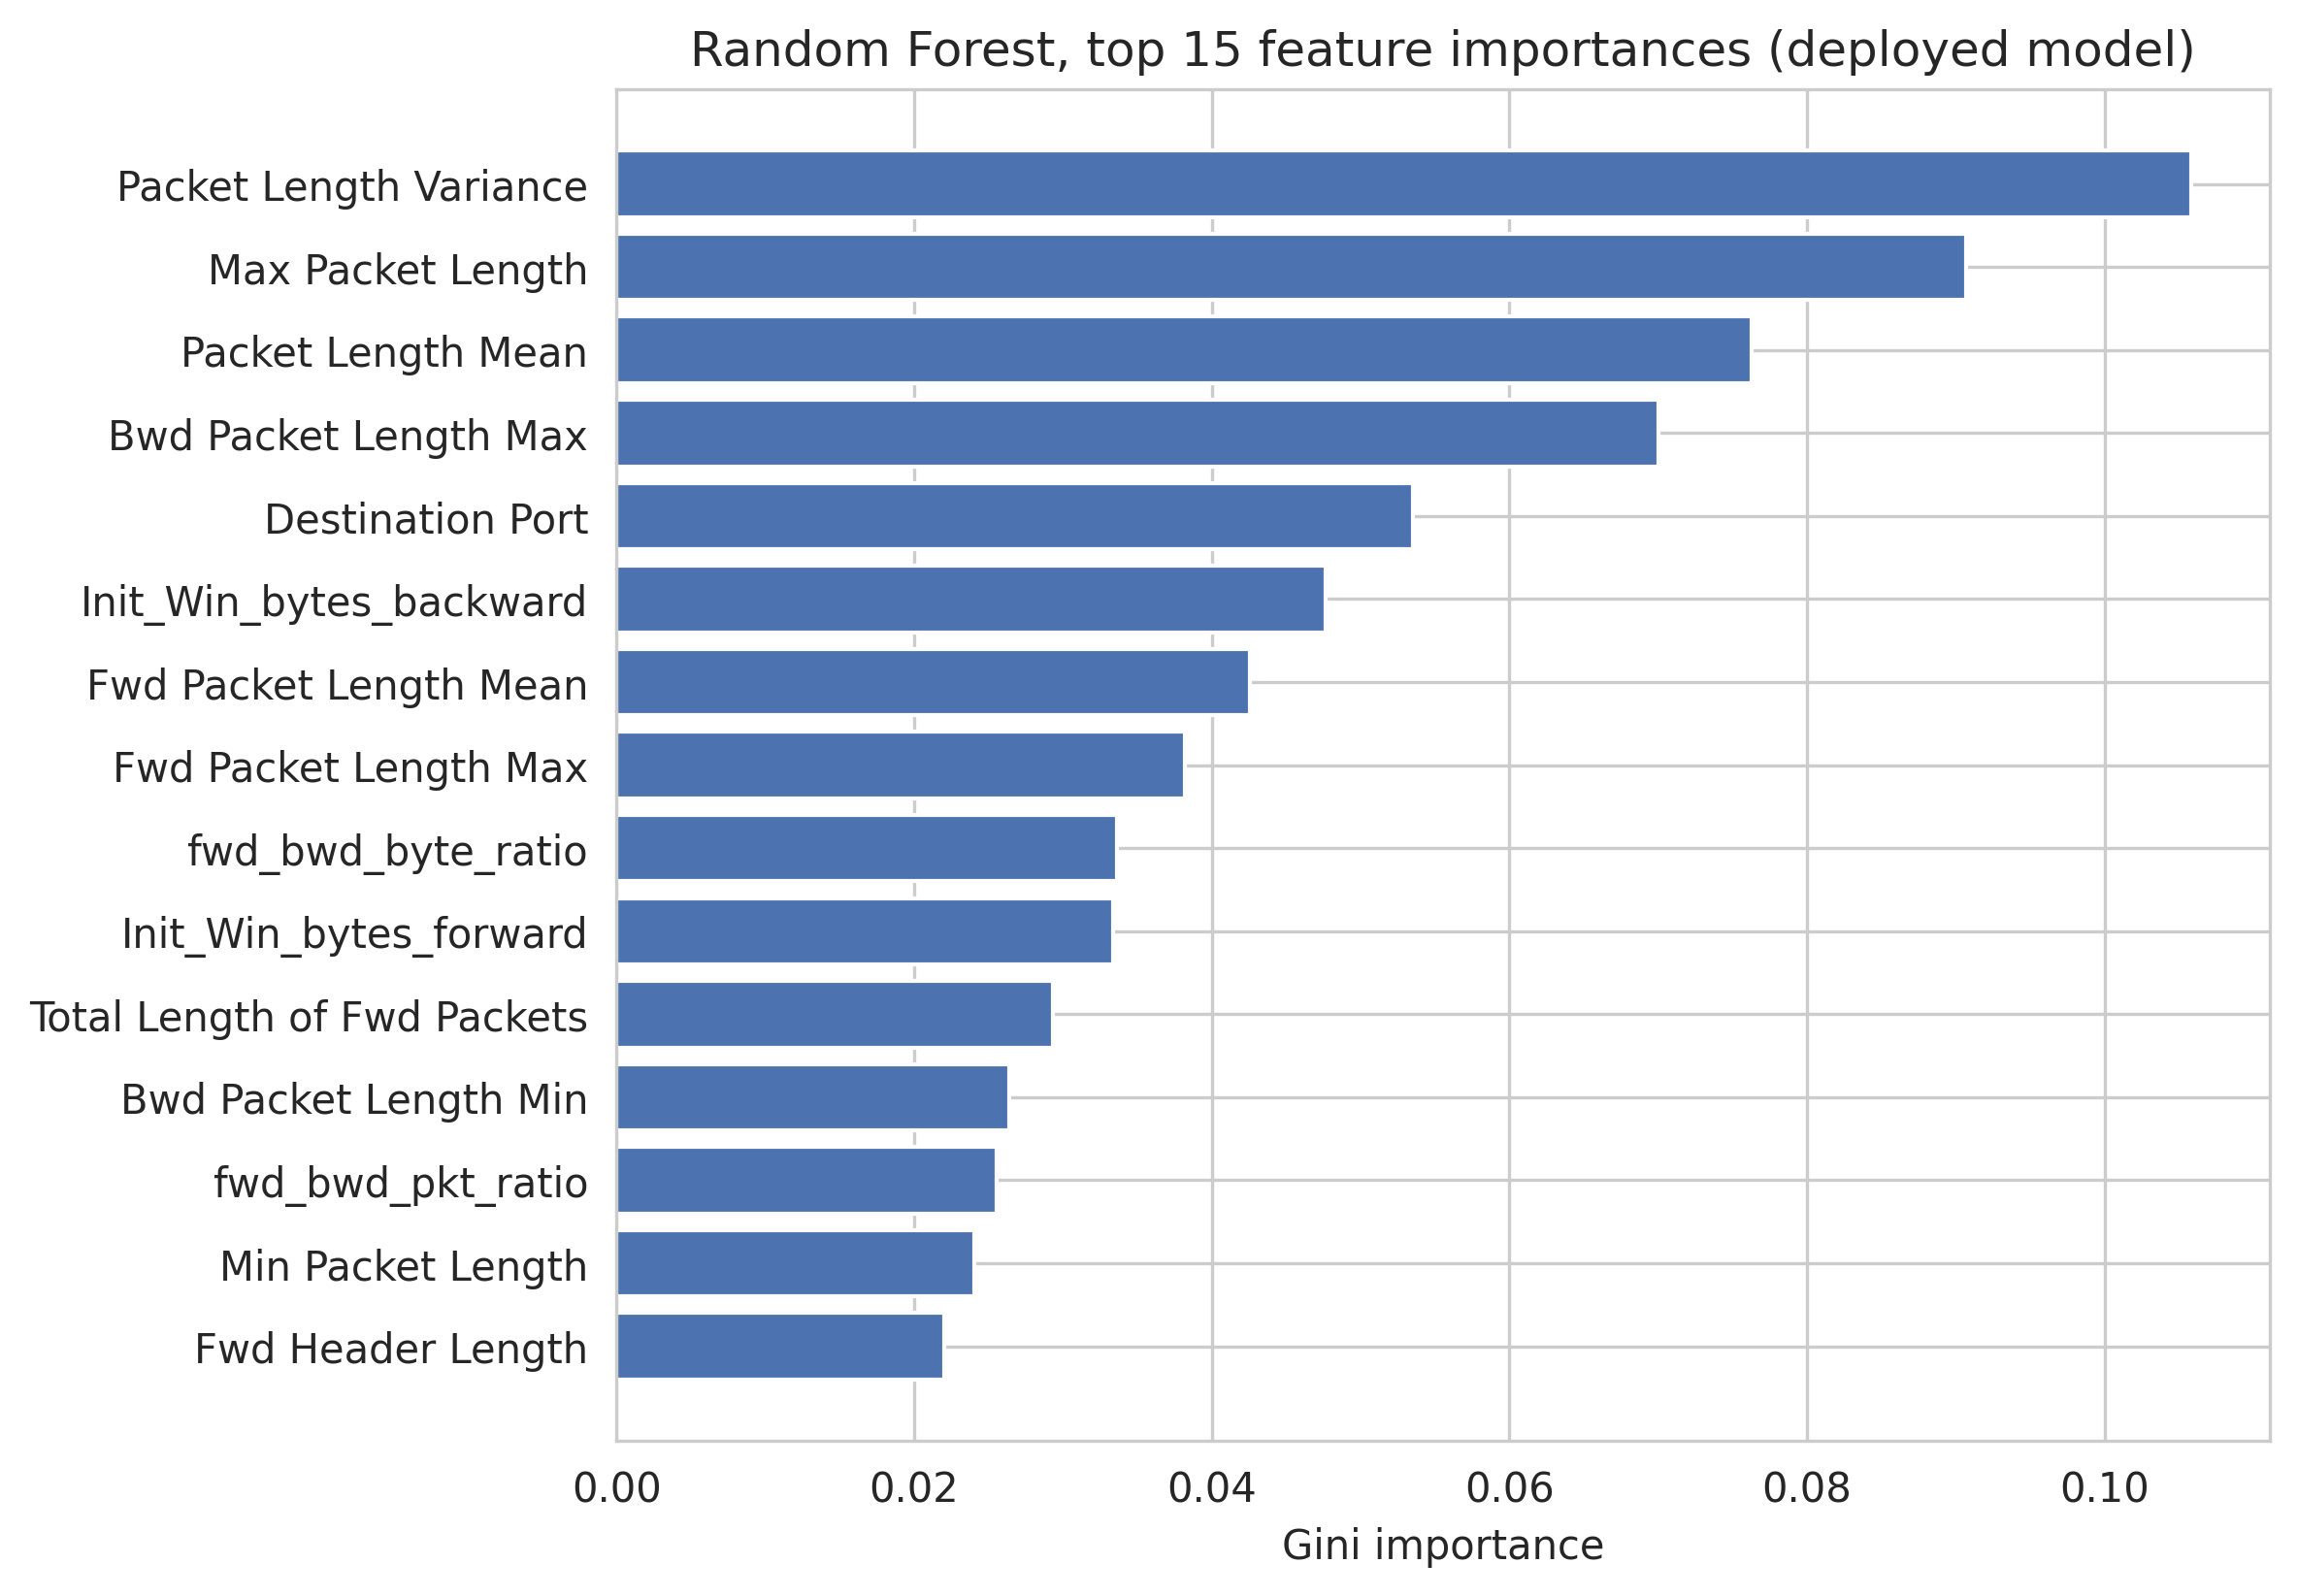
\includegraphics[width=0.85\textwidth]{figures/rf_feature_importance.png}
  \caption{Gini feature importance of the deployed Random Forest, the fifteen highest of its 49 features.}
  \label{fig:rf_importance}
\end{figure}

What SHAP effectively does is apply these ideas to the decision process in such a way as to allow a general view of how vital each feature is to the overall classification. This is what is shown in Figure~\ref{fig:shap} and at the sample size of 2000 test flows, this view agrees with the ordering of importance given by the forest model; the destination port, the forward and backward initial TCP window sizes, and packet-length derived statistics are shown to be most important. In addition, one of the two surviving engineered ratios, the forward to backward byte ratio, appears within the top ten features.

\begin{figure}[H]
  \centering
  \IfFileExists{figures/shap_summary.png}{%
    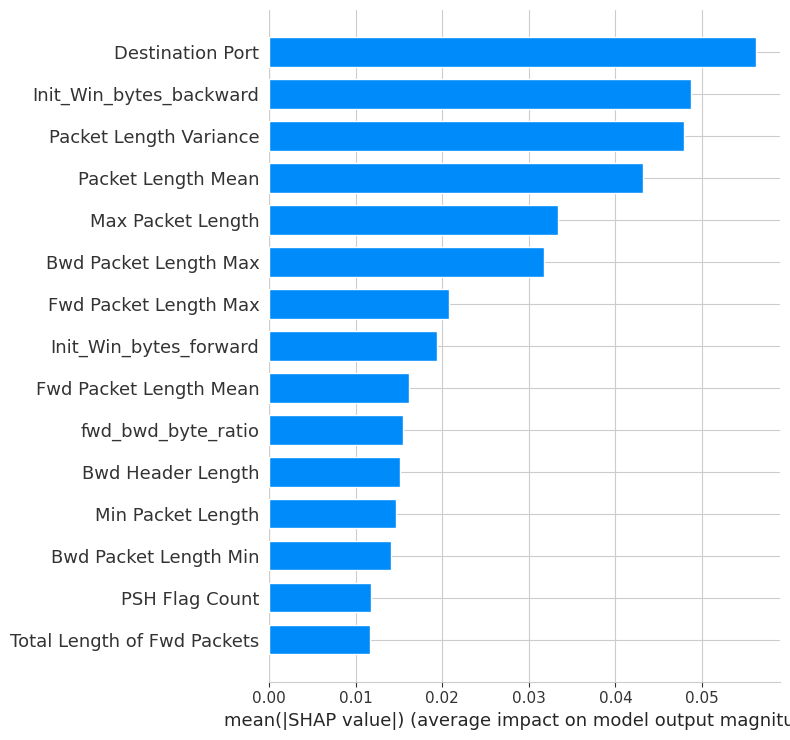
\includegraphics[width=0.85\textwidth]{figures/shap_summary.png}%
  }{%
    \fbox{\parbox{0.85\textwidth}{\centering\vspace{1.0cm}
    \texttt{[Figure: shap\_summary.png]}\\[4pt]
    \small SHAP feature-importance summary over the model's decisions,
    showing which flow features most influence the attack verdict.
    Exported from the training notebook.
    \vspace{1.0cm}}}%
  }
  \caption{SHAP feature importance summary for the trained detector.}
  \label{fig:shap}
\end{figure}


A bar chart orders features by importance, but the impact of a feature can be either positive or negative. Figure~\ref{fig:shap_beeswarm} shows a similar explanation of the data, but with the features ordered as a distribution: each point is a single flow, its horizontal position indicates how much that feature contributed to the verdict for that flow, and the color indicates the value of the feature itself. In this case, we see that the logic of the model is more understandable: a low destination-port value is indicative of an attack, while a high destination port number is indicative of benign traffic.
This matches the pattern in the dataset: attacks tend to be confined to only a handful of service ports, whereas benign traffic utilizes much higher destination port numbers.
We also see that attack flows are more likely to have high packet-length variance, and benign flows are more likely to have a large backward initial window.

This not so related yet dramatic observation requires discussion and should not have been posed as a footnote to the above figure. Destination port turns out to be the single strongest characteristic in both viewpoints, and this is actual information upon which it is reasonable to base this model; yet, also it is the feature most unlikely to be relevant to another network, since it encodes the services being attacked here, not the attack itself. This point is reconsidered in Section~\ref{sec:results_validation} with data from lab traffic.


\begin{figure}[H]
  \centering
  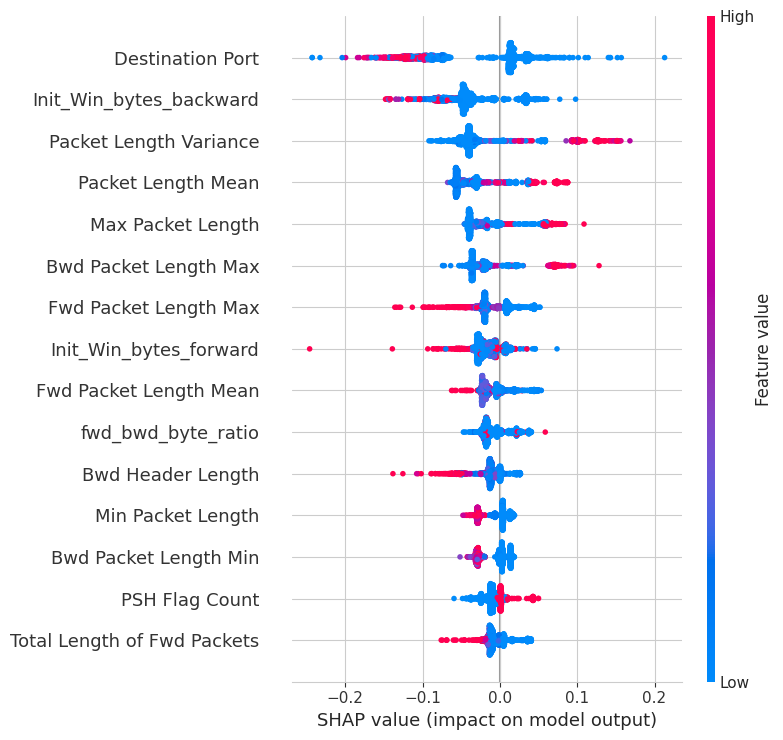
\includegraphics[width=0.85\textwidth]{figures/shap_beeswarm.png}
  \caption{SHAP values for individual flows. Each point is one flow, its colour encodes the value of the feature and its horizontal position the contribution of that feature to the attack verdict.}
  \label{fig:shap_beeswarm}
\end{figure}

In the proposed production system, these explanations would be passed to the analyst on a dashboard, which we discuss in Chapter \ref{chap:conception}. Below we apply the explainability layer to the detector itself; the analyst interface dashboard is omitted in favor of more research.

% ─────────────────────────────────────────────────────────────
\section{Validation on Independently Generated Traffic}
\label{sec:results_validation}

Everything that has been done so far is normal, good practice and culminate in a model that almost succeeds a public benchmark test. We are now faced with the question that a benchmark can not answer alone: will the model identify attacks that come at it in a format that never encountered during training. We tested the model by throwing actual attacks at it in the lab, translating them in the same representation that the model consumes, and then letting the model loose on it. That's where we have our own contribution and that's why its outcome is the only important result of this work as we consider it to be.

\subsection{From benchmark to reality: the feature pipeline}
\label{sec:results_pipeline}

To direct the lab traffic to the model, the lab traffic should first be transformed into a feature vector, i.e. Into the form of features that the model was trained on. The lab traffic is recorded using “tcpdump” in a VM, where we then process it into a flow vector format using CICFlowMeter, the exactly same recording tool as we used when generating the training data. Both the training data and lab traffic data have same definitions regarding the features they should contain.
 
There was one conflict we faced, the training file was generated using a pervious version of CICFlowMeter, the current version has different names for many columns, for example, it write “Dst Port” whereas the old version writes “Destination Port”, etc, although it computes the same quantities based on header values. After verification with both header formats of original and new generated file, we write a “renaming” file which maps current CICFlowMeter column output to original 49-feature model input format. After renaming, we regenerate three computed ratios (as mentioned in features section) exactly the same way it was used for training, and validate the columns of input features file before feeding them to the model. If there is a discrepancy in the input file format and model definition it is detected “loudly” instead of feeding the model something “silently” wrong. This rename step, although simple is in itself an interesting finding, because the very tool which define this benchmark has evolved across versions, this evolution will inevitably appear as “frictions” that a system designed to exceed the benchmarks must overcome.

\subsection{detection results Per-attack}
\label{sec:results_perattack}

The four captures are generated individually so that its corresponding label is clear: a benign browsing session, an SSH brute-force run, a full port scan, and a SYN flood. Since our captures only contain traffic from one type of attack, every flow in each capture is by construction labelled, which is desirable as an analyst might not want to label a million-flow capture. Finally we feed these individual captures through the learned detector and register the percentage of flows it identified in each one, shown in Table~\ref{tab:per-attack-results}.

\begin{table}[H]
  \centering
  \caption{Detection results on independently generated lab traffic.}
  \label{tab:per-attack-results}
  \renewcommand{\arraystretch}{1.3}
  \begin{tabularx}{\textwidth}{Xrrrrr}
    \toprule
    \textbf{Traffic type} & \textbf{Flows} & \textbf{Flagged} & \textbf{Rate (\%)} & \textbf{Mean prob.} & \textbf{Max prob.} \\
    \midrule
    Benign traffic     & 21            & 0 & 0.00  & 0.148 & 0.160 \\
    SSH brute force    & 6             & 4 & 66.67 & 0.488 & 0.695 \\
    Port scan          & 65,537        & 0 & 0.00  & 0.000 & 0.270 \\
    SYN flood (DoS)    & 1,523,389     & 0 & 0.00  & 0.058 & 0.150 \\
    \bottomrule
  \end{tabularx}
\end{table}

Another thing to note is that each capture was recorded separately, meaning the attack type acts as a ground-truth label on each flow. The benign row therefore reports false positives, while the attack rows report detections. The model did not identify any on the benign traffic which means no false positives on this dataset.

The last two columns show the attack probability the model assigned, not only the decision it reached. This is interesting because it shows that the misses are nowhere near the decision threshold. On a review of over 1.5 million flood flows, the maximum attack probability was 0.150 and for 65,537 scan flows, was 0.270.
These are well below the decision threshold of 0.5, and the operating point of 0.340 of Table~\ref{tab:operating_points}.
As such, these false negatives would not have been recovered, even if the threshold was reduced. There appears to be no hesitation in relation to the traffic, the model clearly has confidence that it is benign.

The proposed detector is being effective by not forcing false alarms and thus, not mistakenly classifying the normal network traffic as malicious activity. The previous statement refers to the criticism of the operation noise as the second part of Chapter~\ref{chap:ids} concerning the false alarms that commercial detectors create when carrying out their normal work.

Regarding \textbf{SSH brute force} the model correctly predicted four of six flows. This number should be considered a qualitative estimate rather than quantitative since the sample size of six flows is very small. The trend in the results though is most important as this was the only type of attack to demonstrate any transferability at all.
The reason is most likely structural.
The brute-force attack class in the training data consisted of complete login sequences, and the Hydra traces look similar to this training data. Enough similarity is preserved for the model to react, albeit weakly, with its confidence marginally above the decision threshold.

This pairing of the detector with an explainer allows an investigation into how a flow is being flagged instead of simply recording that it has been flagged. Figure~\ref{fig:shap_local} employs the SHAP layer outlined in Section~\ref{sec:results_shap} to examine the top-scoring brute-force flow, and this explanation extends the previous text. The most important factor contributing to the change of moving the base value 0.5 to the verdict of 0.695 is that the destination port is 22, whereas the packet-shape features oppose this.
This indicates that the similarity that makes this transfer attack possible is mostly due to the port – strongly linked to attacks within the training set – rather than the shape of the authentication exchange.
Also, this is the first working demonstration of the alerting behaviour designed in Section~\ref{sec:conception_realtime}, where an alert arrives with its explanation attached, in terms of the flow features that produced it.

\begin{figure}[H]
  \centering
  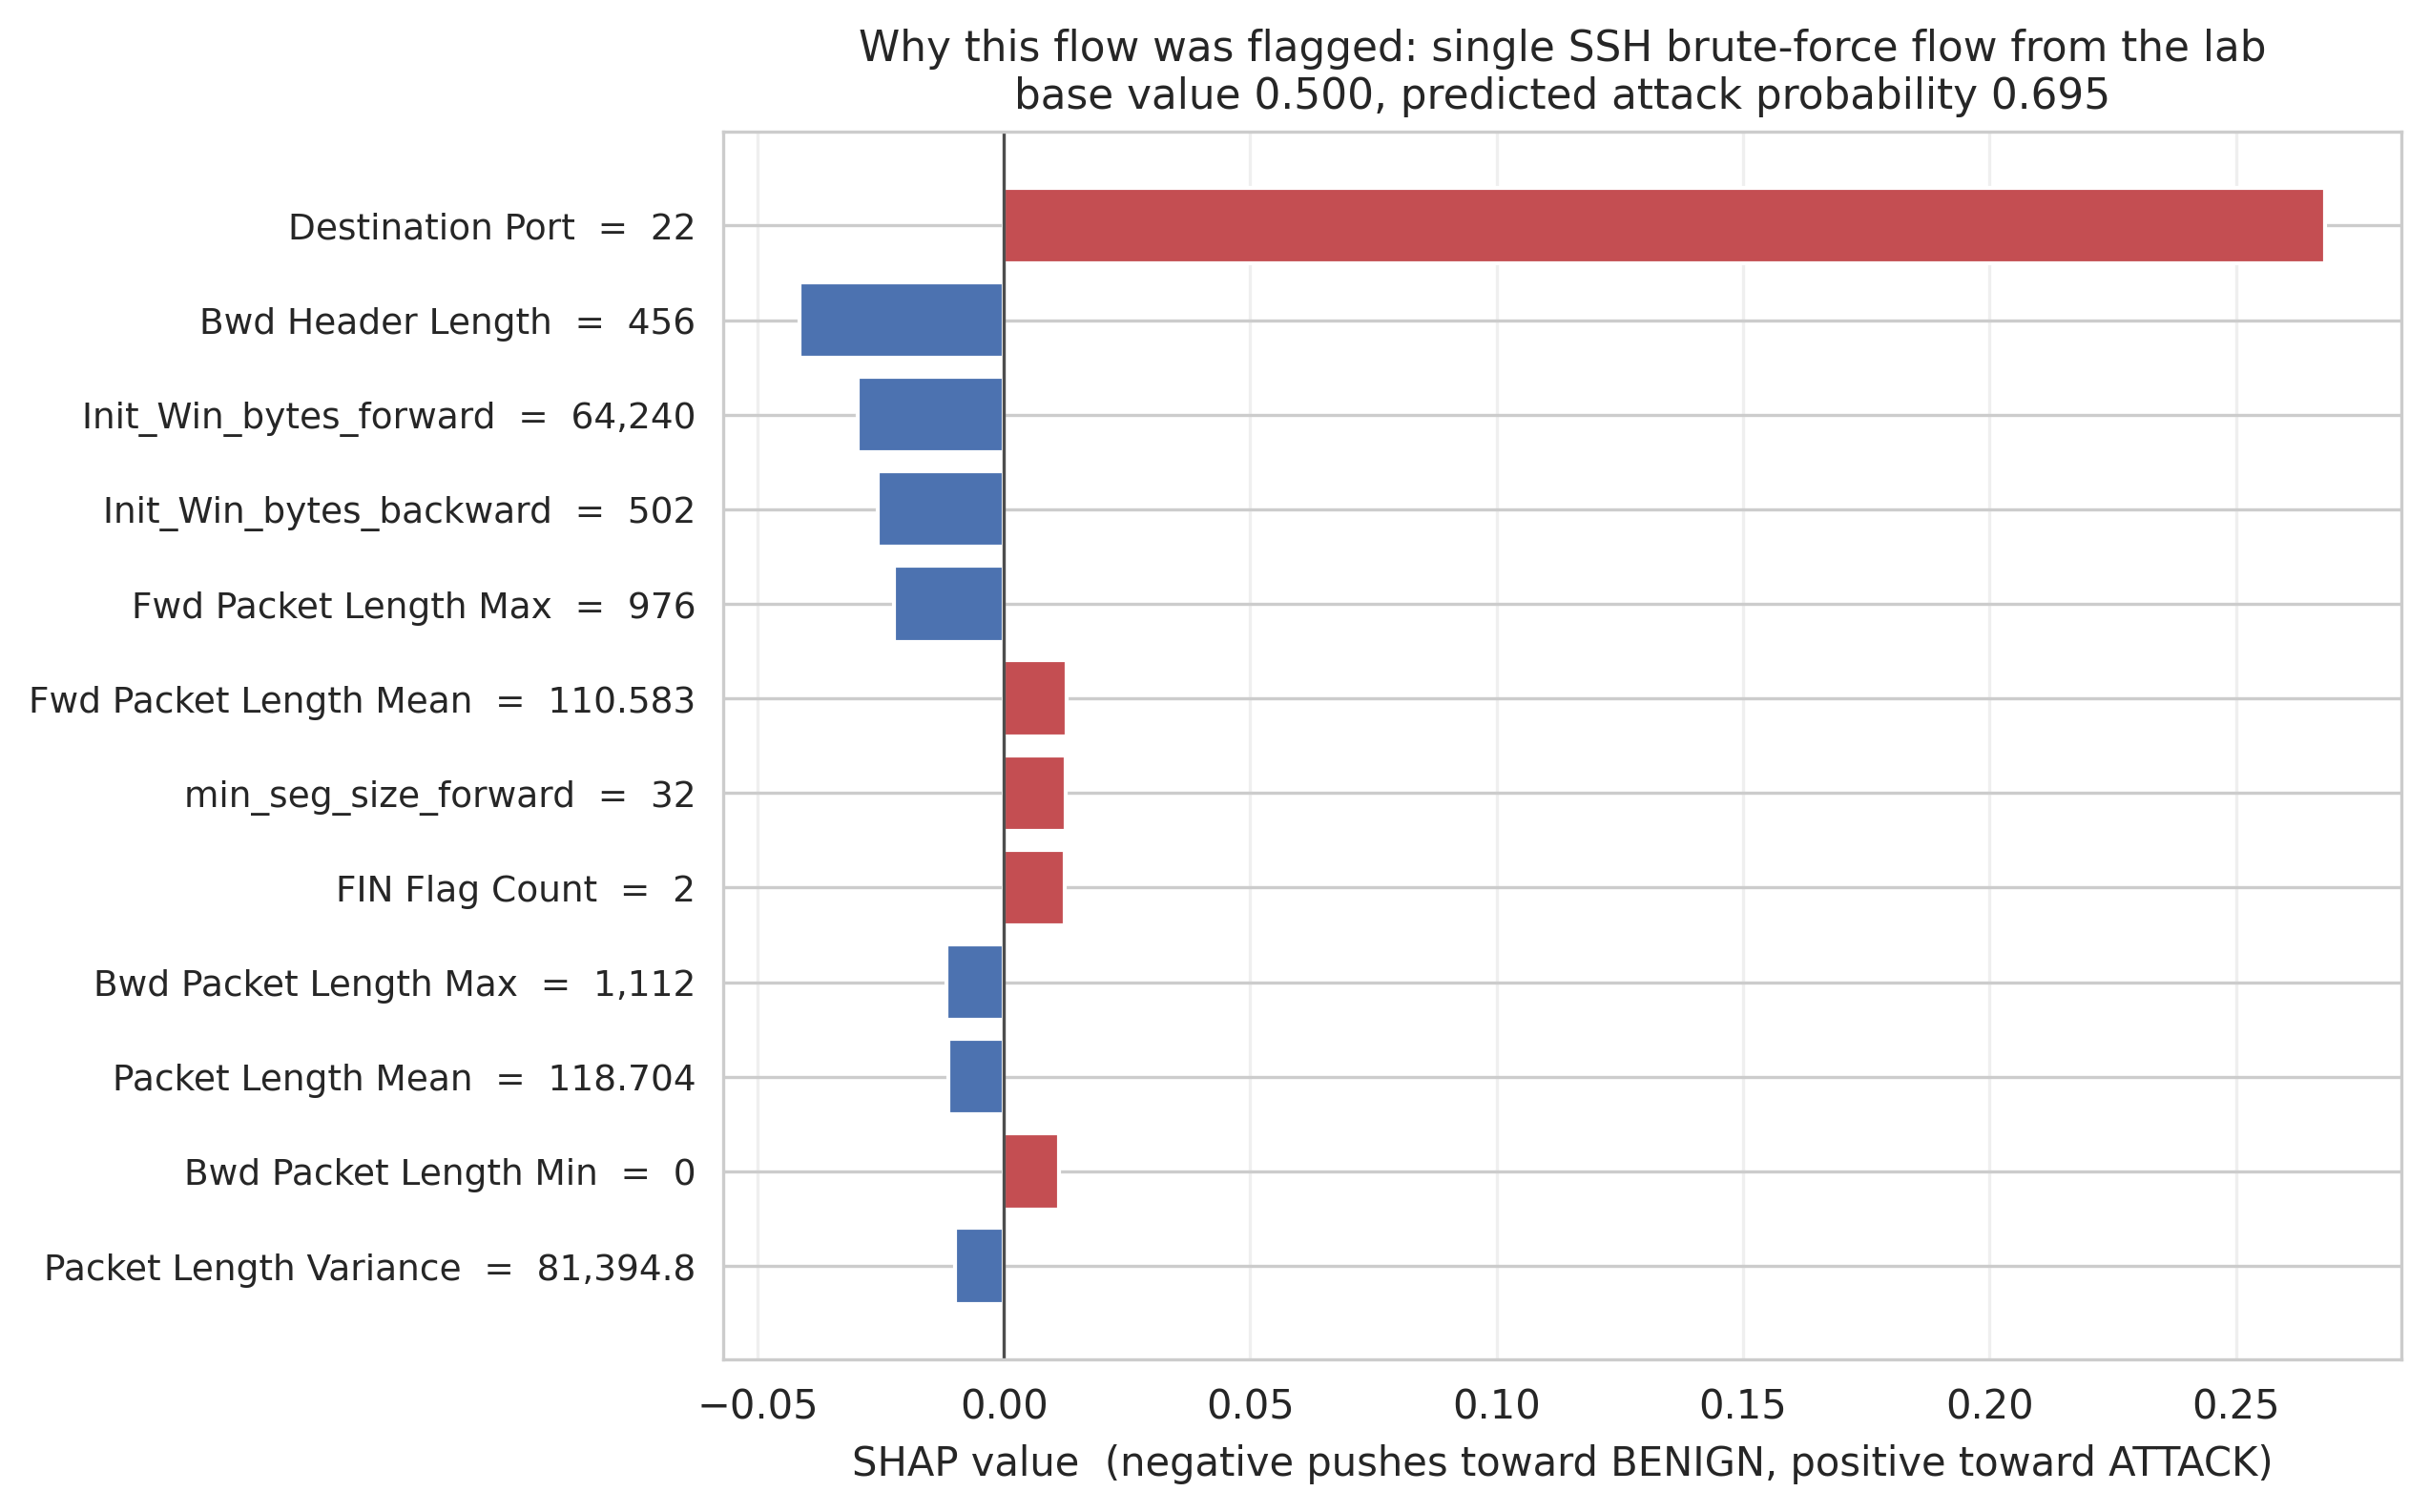
\includegraphics[width=0.9\textwidth]{figures/shap_local_ssh_flow.png}
  \caption{Per-alert explanation for one flagged SSH brute-force flow from the laboratory. Red bars push the verdict toward attack, blue bars toward benign.}
  \label{fig:shap_local}
\end{figure}

The model was entirely blind to both the \textbf{port scan} and the \textbf{SYN flood}, reporting zero detections across all sixty-five thousand scan flows and zero across the more than one and a half million flood flows. These are not marginal misses; they are total. A model that scores $0.997$ on the benchmark detected none of two high-volume attacks generated a few metres away. Understanding why is the focus of the section that follows.

\subsection{Analysis of the generalization gap}
\label{sec:results_gap}

This failure is not arbitrary, nor is it a bug in the pipeline - the features were computed and aligned correctly and valid data was passed to the model; there's a single clear reason for the failure, and the failure teaches us something about benchmarks, not this specific model.

Another example of a flow representation is SYN flood or port scan, which consists of only one packet sent to a target that does not connect. A single packet with a SYN flag, no reply, zero duration, 1 forward direction, and zero backward direction. CICFlowMeter correctly classifies both cases as flow, and therefore a million-packet SYN flood generates a million one-packet flows, mostly empty.
Impact of the training data It is interesting to note that application-level floods in the training data from CICIDS-2017 involve finished connections with application level requests and responses, multi-packet flows, a finite duration and specific rates. Therefore a denial of service attack will be more likely to follow this pattern. On the other hand, single packet SYN without duration looks like a very short benign connection stub that is likely to be allowed by this system.

There is, from the evidence found, a difference between the hping3 SYN flood and the DoS attack CICIDS-2017, even though the former has been provided as an identifier of the latter in the operation level in which the model works. The same is observed in the case of port scans, where the nmap SYN scan differs from the one used in the benchmarks, as the flow was built differently and the model was trained on it.
The one sentence in English that contains all rows in Table~\ref{tab:per-attack-results} is: The model can recognize attacks whose properties are expressed by rich multi-packet flows but cannot recognize attacks whose properties are expressed by slim single-packet flows. Further, this sentence also explains the benign cases, the partial-transfer of SSH, and the two total omissions.

\begin{figure}[H]
  \centering
  \IfFileExists{figures/generalization_gap.png}{%
    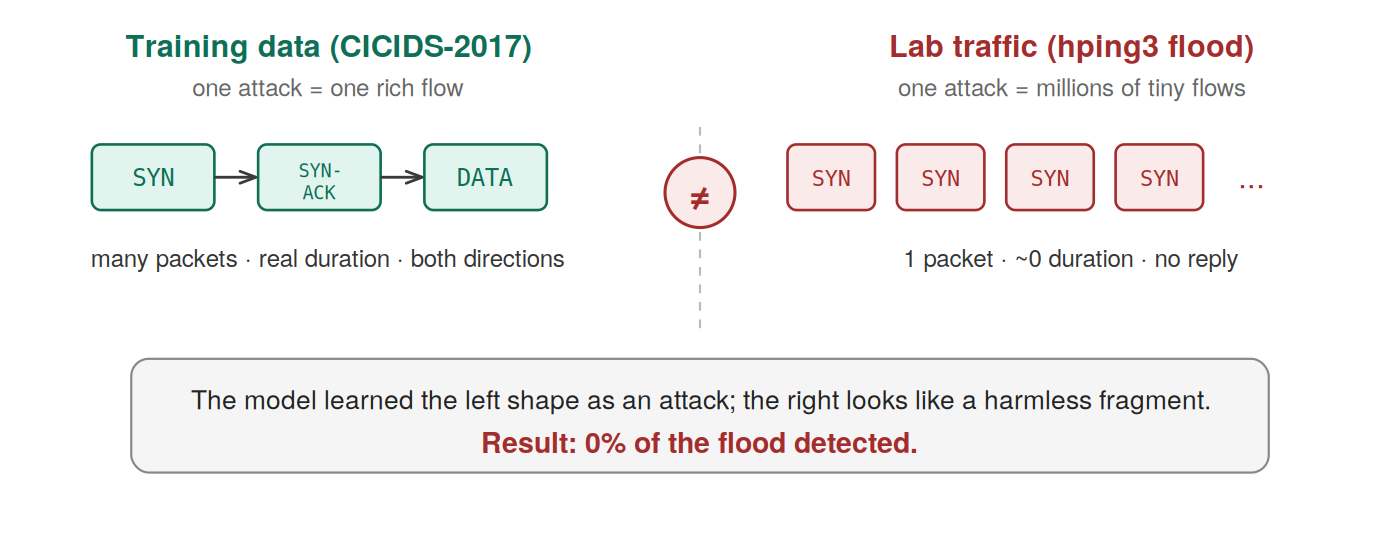
\includegraphics[width=0.95\textwidth]{figures/generalization_gap.png}%
  }{%
    \fbox{\parbox{0.85\textwidth}{\centering\vspace{1.0cm}
    \texttt{[Figure: generalization\_gap.png]}\\[4pt]
    \small Why the volumetric attacks were missed. Training taught
    ``DoS = rich multi-packet HTTP flood''; the lab produced
    single-packet SYN floods with near-zero duration. Same name,
    different flow structure, hence no detection.
    \vspace{1.0cm}}}%
  }
  \caption{The generalization gap: benchmark attacks and lab attacks that share a name but not a flow structure.}
  \label{fig:gen_gap}
\end{figure}

Our findings seem to establish that the current work has yielded important results. In particular, that we have recreated with traffic data traces owned by us one of the most well-known weaknesses of benchmark-trained intrusion detection systems: that high benchmark performance may not be indicative of high performance in real systems. While this argument has been made before in the research literature, in this work we have validated its occurrence, quantified its extent over a range of attacks, and traced it to a particular problem with flow representation.

% ─────────────────────────────────────────────────────────────
\section{Discussion}
\label{sec:results_discussion}

The result can be divided into 2 categories. The successful and unsuccessful approach. Based on the result, the model has been able to choose the most efficient and accurate model and achieved a state-of-the-art score on the benchmark.
Additionally, the model does not give any false positive on the benign traffic captured in the laboratory, while also providing explanations to its prediction with SHAP.
One disadvantage of the model is that it does not identify the volumetric attack we generate and we do know why.

There is one identified specific solution and one generic non-specific solution, but there could be any number of other solutions. The results indicate that precisely the flood that the learned classifier misses is one that other mechanisms can detect easily. For example, one could characterize the flood of single-packet SYN packets from a single host by their sending rate, and set a rule to raise an alarm whenever there are N half-open connections/sec from a source address.
This rule would quickly detect the flood missed by the learned classifier.
Therefore, the best designs is probably a \emph{hybrid} design, combining the learned classifier for the structural attacks for which it currently works well, and a set of simple rate-based rules for the volumetric attack with large packet volume. Such hybrid designs have been used in more sophisticated detectors, and the per-attack results above indicate why the combination would be effective here.

A second solution is to bypass the training gap directly retraining not just on the benchmark but also on some of lab generated traffic. As automatically taken snapshots are obviously annotated by definition, constructing a training set from these does not require humans to go through and classify them and should result in better detection of the exact types of attack that we are failing on. It is a straight forward step forward not a new experiment.

The remaining outstanding element the streaming deployment that is described in Chapter~\ref{chap:conception} i.e. The message bus, the real-time detection service and the analyst console. Our throughput achieved about 45k of flows per second that suggests a real-time operation in practice could be achievable, with the engineering outstanding.

% ─────────────────────────────────────────────────────────────
\section{Summary}
\label{sec:results_summary}

The design outlined in chapter \ref{chap:conception} has been successfully applied and tested in this chapter. We have constructed the two-machine lab, cleaned and set up the CICIDS-2017 data, developed and picked out a representation that only uses 49 features, and selected the best from three potential model approaches. One surprising aspect of the experimental results, when compared with a prior belief about the appropriate learning model, is that a Random Forest is better than a CNN or LSTM approach for this problem and the model resource usage is considerably lower. With above near perfect classification on the benchmark data and interpretation from SHAP explaining the classification decisions, we recommend this model for future efforts.

Finally, we took that model and subjected it to the only test that we felt really mattered: experiments on a set of our own attack and benign traffic data. That model generated zero false alarms and somewhat detected SSH brute-force, but completely failed to detect both a portscan and a SYN flood, because (as flow data) neither of them has the least similarity with the kind of multi-packet attacks that were in the training set. This conclusion is arguably the main contribution of our paper: proof on our own dataset that benchmark detection performance and detection on "real" data are vastly different, and a "fix" for this problem (a rule-based hybrid method, learned from the data).
